\documentclass[11pt,a4paper]{article}
\usepackage[margin=22mm,top=19mm,bottom=19mm]{geometry}
\usepackage{fontspec}\setmainfont{Cambria}\setsansfont{Calibri}\setmonofont{Consolas}[Scale=.9]
\usepackage{amsmath,amssymb,graphicx,booktabs,array,xcolor}
\setlength{\parindent}{0pt}\setlength{\parskip}{6pt}\setlength{\emergencystretch}{2em}
\renewcommand{\arraystretch}{1.18}\setlength{\tabcolsep}{5pt}
\newcommand{\heading}[2]{{\sffamily\small\color{blue!40!black}#1}\par{\sffamily\LARGE\bfseries#2}\par\vspace{3mm}}
\newcommand{\page}[2]{\newpage\heading{#1}{#2}}
\begin{document}
\heading{Güncellenmiş proje modeli | 22 Eylül 2026}{Altı gereksinim seviyesi\\Düşünme, inceleme ve karar döngüsü}
\textbf{İstenen akış.} Siyah-beyaz resmin ilk satırı \textbf{1. seviye
gereksinim} olarak işaretlenir. Ardından aşağı doğru büyüyen on satır
\textbf{düşünme ve inceleme dönemi} olur. Bir sonraki satırda yeni gereksinim
seviyesi ve entropiyi azaltan karar gösterilir. Bu döngü, 6. seviyede sıfır
açık karar belirsizliğine ulaşıncaya kadar beş kez tekrarlanır.

\begin{center}\begin{tabular}{cll}\toprule
Adım $t$ & Satırın adı & İşlem\\\midrule
0 & 1. seviye gereksinim & Başlangıç kodlaması\\
1--10 & Düşünme ve inceleme 1 & 10 genişleme adımı\\
11 & 2. seviye gereksinim & Karar ve yeniden kodlama\\
12--21 & Düşünme ve inceleme 2 & 10 genişleme adımı\\
22 & 3. seviye gereksinim & Karar ve yeniden kodlama\\
23--32 & Düşünme ve inceleme 3 & 10 genişleme adımı\\
33 & 4. seviye gereksinim & Karar ve yeniden kodlama\\
34--43 & Düşünme ve inceleme 4 & 10 genişleme adımı\\
44 & 5. seviye gereksinim & Karar ve yeniden kodlama\\
45--54 & Düşünme ve inceleme 5 & 10 genişleme adımı\\
55 & 6. seviye gereksinim & Son seçim ve kabul; $U=H_1=0$\\\bottomrule
\end{tabular}\end{center}
Başlangıç $t=0$ olarak sayılır. Dolayısıyla 55 geçiş ve başlangıç dahil
56 satır vardır. Karar satırı da sola ve sağa birer beyaz hücre eklenerek
genişler; bu satırda fazladan bir düşünme kuralı çalıştırılmaz.

\textbf{Beş ayrı deney.} Sıralı karar, paralel çalışma, kısıt yayılımı,
kanıt güncellemesi ve prototip elemesi aynı zaman çizelgesinde ayrı ayrı
çalıştırılır. Yöntemler peş peşe tek resimde birleştirilmez; her birinin
altı seviyeli resmi, karar tablosu ve entropi grafiği vardır.

\textbf{Deneyin statüsü.} Bu bir başarı senaryosu simülasyonudur. Nihai
kabul sonuçları varsayımsal girdidir; fiziksel test yapılmış sayılmaz.
Sıfır, tanımlı proje kapsamındaki açık kararların kapanmasıdır.

\page{Ortak gereksinim}{1\quad Cümleden alternatiflere}
\begin{quote}\itshape
``Kapı mekanizması, ilkokul çağındaki bir çocuğun bile hiç zorlanmadan tek
eliyle açıp kapatabileceği bir tasarıma sahip olmalıdır.''
\end{quote}
Önceki raporun $\mathbf x_0=011101000$ satırı korunmuştur. Siyah işaretler
yaş kapsamı (A), referans profil (B), kuvvet sınırı (C) ve işlev kapsamı (D)
konularına karşılık gelir. Başlangıçta her konu iki seçeneklidir:
\begin{center}\small\begin{tabular}{c p{56mm} p{66mm}}\toprule
Konu & 0 seçeneği & 1 seçeneği\\\midrule
A & 8--12 yaş kapsamı & 6--12 yaş kapsamı\\
B & P0 küçük el referans fikstürü & P1 orta el referans fikstürü\\
C & 15 N tasarım hedefi & 10 N tasarım hedefi\\
D & Yalnız mandal çözme & Tam açma ve kapama\\\bottomrule
\end{tabular}\end{center}
Bu sayılar ve fikstürler örnek tasarım girdileridir; çocuklara uygunluk veya
standartlara uyum sonucunu temsil etmez. P0/P1 çizimleri ile test koşullarının
gerçek projede ayrıca tanımlanması gerekir.

\textbf{Paket ve resim farklı kodlardır.} ABCD biçiminde 16 paket bulunur;
başlangıçta hepsi $1/16$ ağırlıktadır. Hedef paket 1011'dir. Paketteki 0,
bir alternatifin kimliğidir. Resimdeki beyaz ise işaret bulunmayan hücredir.
Karar sonrasında siyah hücreler artık tek tek kelimeleri değil, karar
kaydına bağlı \emph{özetlenmiş açık konu işaretlerini} gösterir.

\textbf{Gereksinim seviyesinin içeriği.} Her seviye bir cümle ile birlikte
seçilmiş seçenekler, hâlâ açık seçenekler ve kabul koşullarını içerir.
2--5. seviyelerde bazı ifadeler tercih veya aday olarak kalabilir. Hangi
konunun hangi seviyede kesinleştiği beş yöntemin karar tablolarında ayrıdır.

\textbf{6. seviye için ortak sonuç cümlesi:}
\begin{quote}
Proje, 6--12 yaş kapsamını esas alacaktır. Tanımlı P0 referans fikstüründe,
tepe işletme kuvveti 10 N'yi aşmadan, tek elle mandalın çözülmesi, kapının
$0^\circ$'den $90^\circ$'ye açılması ve yeniden kapatılması sağlanacaktır.
\end{quote}
Kapsam onayı, P0/test prosedürü onayı, kuvvet doğrulaması ve tam işlev
doğrulaması dört kabul kaydıdır. Simülasyonda bunların $t=55$'te geçtiği
varsayılır; gerçek bir test başarısızsa 6. seviye tamamlandı sayılamaz.

\page{Düşünme dönemlerinin anlamı}{2\quad On adımda ne inceleniyor?}
Hücresel otomat, bir düşünme döneminde ilişkilerin yayılmasını gösteren
sembolik bir modeldir. On satır on gerçek gün veya ölçülmüş zihinsel işlem
değildir. Aşağıdaki on faaliyet, bu satırlara karşılık gelebilecek çalışma planıdır:
\begin{center}\small\begin{tabular}{c p{128mm}}\toprule
Yerel adım & Örnek çalışma\\\midrule
1 & Önceki gereksinim seviyesini ve açık konuları oku.\\
2 & Kullanım bağlamını ve sınırlarını incele.\\
3 & Eksik tanımları ve varsayımları listele.\\
4 & Seçenekler arasındaki bağımlılıkları çıkar.\\
5 & Alternatif tasarım veya test yaklaşımı üret.\\
6 & Basit hesap, çizim veya masaüstü model kur.\\
7 & Model çıktısını gereksinimle karşılaştır.\\
8 & Çelişki, eksik kanıt ve uygulanabilirlik sorunlarını incele.\\
9 & Karar için adayları ve gerekçeleri hazırla.\\
10 & İnceleme kaydını tamamla; yeni seviye kararına girdi ver.\\\bottomrule
\end{tabular}\end{center}
Her dönemin sonunda bu çalışmaların varsayımsal çıktısı yöntemine göre
aday ağırlığını, kısıtları veya seçilen paketi günceller. Yalnız hücresel
otomatın çalışması adayları kendiliğinden doğrulamaz.

\textbf{Karşılaştırma için ortak kural dizisi.}
\begin{center}\begin{tabular}{cll}\toprule
Dönem & Adımlar & Kural ve görsel benzetme\\\midrule
1 & 1--10 & 90: iki komşu arasındaki farkı yayma\\
2 & 12--21 & 150: merkez dahil ilişkileri birleştirme\\
3 & 23--32 & 30: asimetrik seçenek etkileşimi\\
4 & 34--43 & 110: yapıların etkileşimi\\
5 & 45--54 & 90: son ilişkileri yeniden inceleme\\\bottomrule
\end{tabular}\end{center}
Bütün yöntemler aynı sırayı kullanır. Kural numaraları yetenek veya düşünme
kalitesi puanı değildir. Dış bölge beyazdır; hücreler eşzamanlı güncellenir.
Karar satırlarında yerel kural yerine bir sonraki bölümdeki karar operatörü vardır.

\page{İki entropi, açık bir gösterim kuralı}{3\quad Seviye geçişinde azalış nasıl sağlanır?}
\textbf{Seçenek entropisi.} Karar kaydındaki paket olasılıklarından
$U_t=-\sum_a p_t(a)\log_2p_t(a)$ hesaplanır. Başlangıçta $U_0=4$ bittir.
Düşünme döneminde $p_t$ sabit tutulur; güncelleme yalnız karar satırında yapılır.
Bu yüzden $U_t$ merdiven biçimindedir. İnceleme sırasında yeni olasılık
kanıtı veya yeni konu eklemek bu sürümün kapsamı dışındadır.

\textbf{Resim entropisi.} Siyah sayısı $b$, genişlik $N=9+2t$ ise
$H_1=h_2(b/N)$ ve $h_2(q)=-q\log_2q-(1-q)\log_2(1-q)$.
Renk entropisi yalnız karar seçimiyle her zaman azalmaz. Bu nedenle istenen
grafik akışı için \emph{entropi kontrollü yeniden kodlama} açıkça tanımlanır.

\textbf{Karar öncesi satır.} Önceki satırın iki yanına birer beyaz hücre
eklenir. Bu geçici satırın entropisi $H_{\rm ön}$, bir önceki düşünme
satırının entropisi $H_{t-1}$, önceki gereksinim seviyesininki $H_{\rm sev}$ olsun.
Yeni olasılıklar hesaplandıktan sonra gösterim hedefi:
\[
H^*=\min(H_{\rm ön},H_{t-1},H_{\rm sev})\frac{U_t}{U_{t-1}}.
\]
Son seviye dışında, mevcut $b$ siyah işaret arasından $k$ işaret korunur.
$1\le k\le\min(b,\lfloor N/2\rfloor)$ ve
\[
h_2(k/N)<\min(H_{\rm ön},H_{t-1},H_{\rm sev})
\]
koşuluyla, hedefi aşmayan en büyük $k$ seçilir. Sonlu hücre sayısı nedeniyle
hedefe ulaşılamıyorsa sıkı azalış sağlayan en küçük $k$ kullanılır. Böyle bir
$k$ da yoksa kod hata verir; sessizce sıfır üretmez. Son seviyede $U=0$ ile $k=0$ olur.

Korunacak konumlar, mevcut siyah konumlar arasından düzenli aralıklarla seçilir.
Bu özetleme aday kaydını değiştirmez; kalan tüm açık konular o kayıtta tutulur.
Resimden silinen bir işaret, tek başına mühendislik probleminin çözüldüğü anlamına gelmez.
Dolayısıyla grafikteki kontrollü azalış bir \emph{gösterim tasarımıdır}; bağımsız başarı kanıtı değildir.

\textbf{Geçmiş korunur.} Bütün geçerli satırlar biriktirilir:
$A_t=(t+1)(9+t)$, $B_t=\sum_{s=0}^t b_s$,
$H_{\rm geçmiş}=h_2(B_t/A_t)$. $t=55$'te 119 hücrelik son satır sıfırdır;
3584 hücrelik geçmişte önceki siyahlar kalır. Geçmişin entropisinin sıfır olması beklenmez.

\page{Yöntem 1/5 | İşaretli siyah-beyaz akış}{Sıralı karar kapıları}
\begin{center}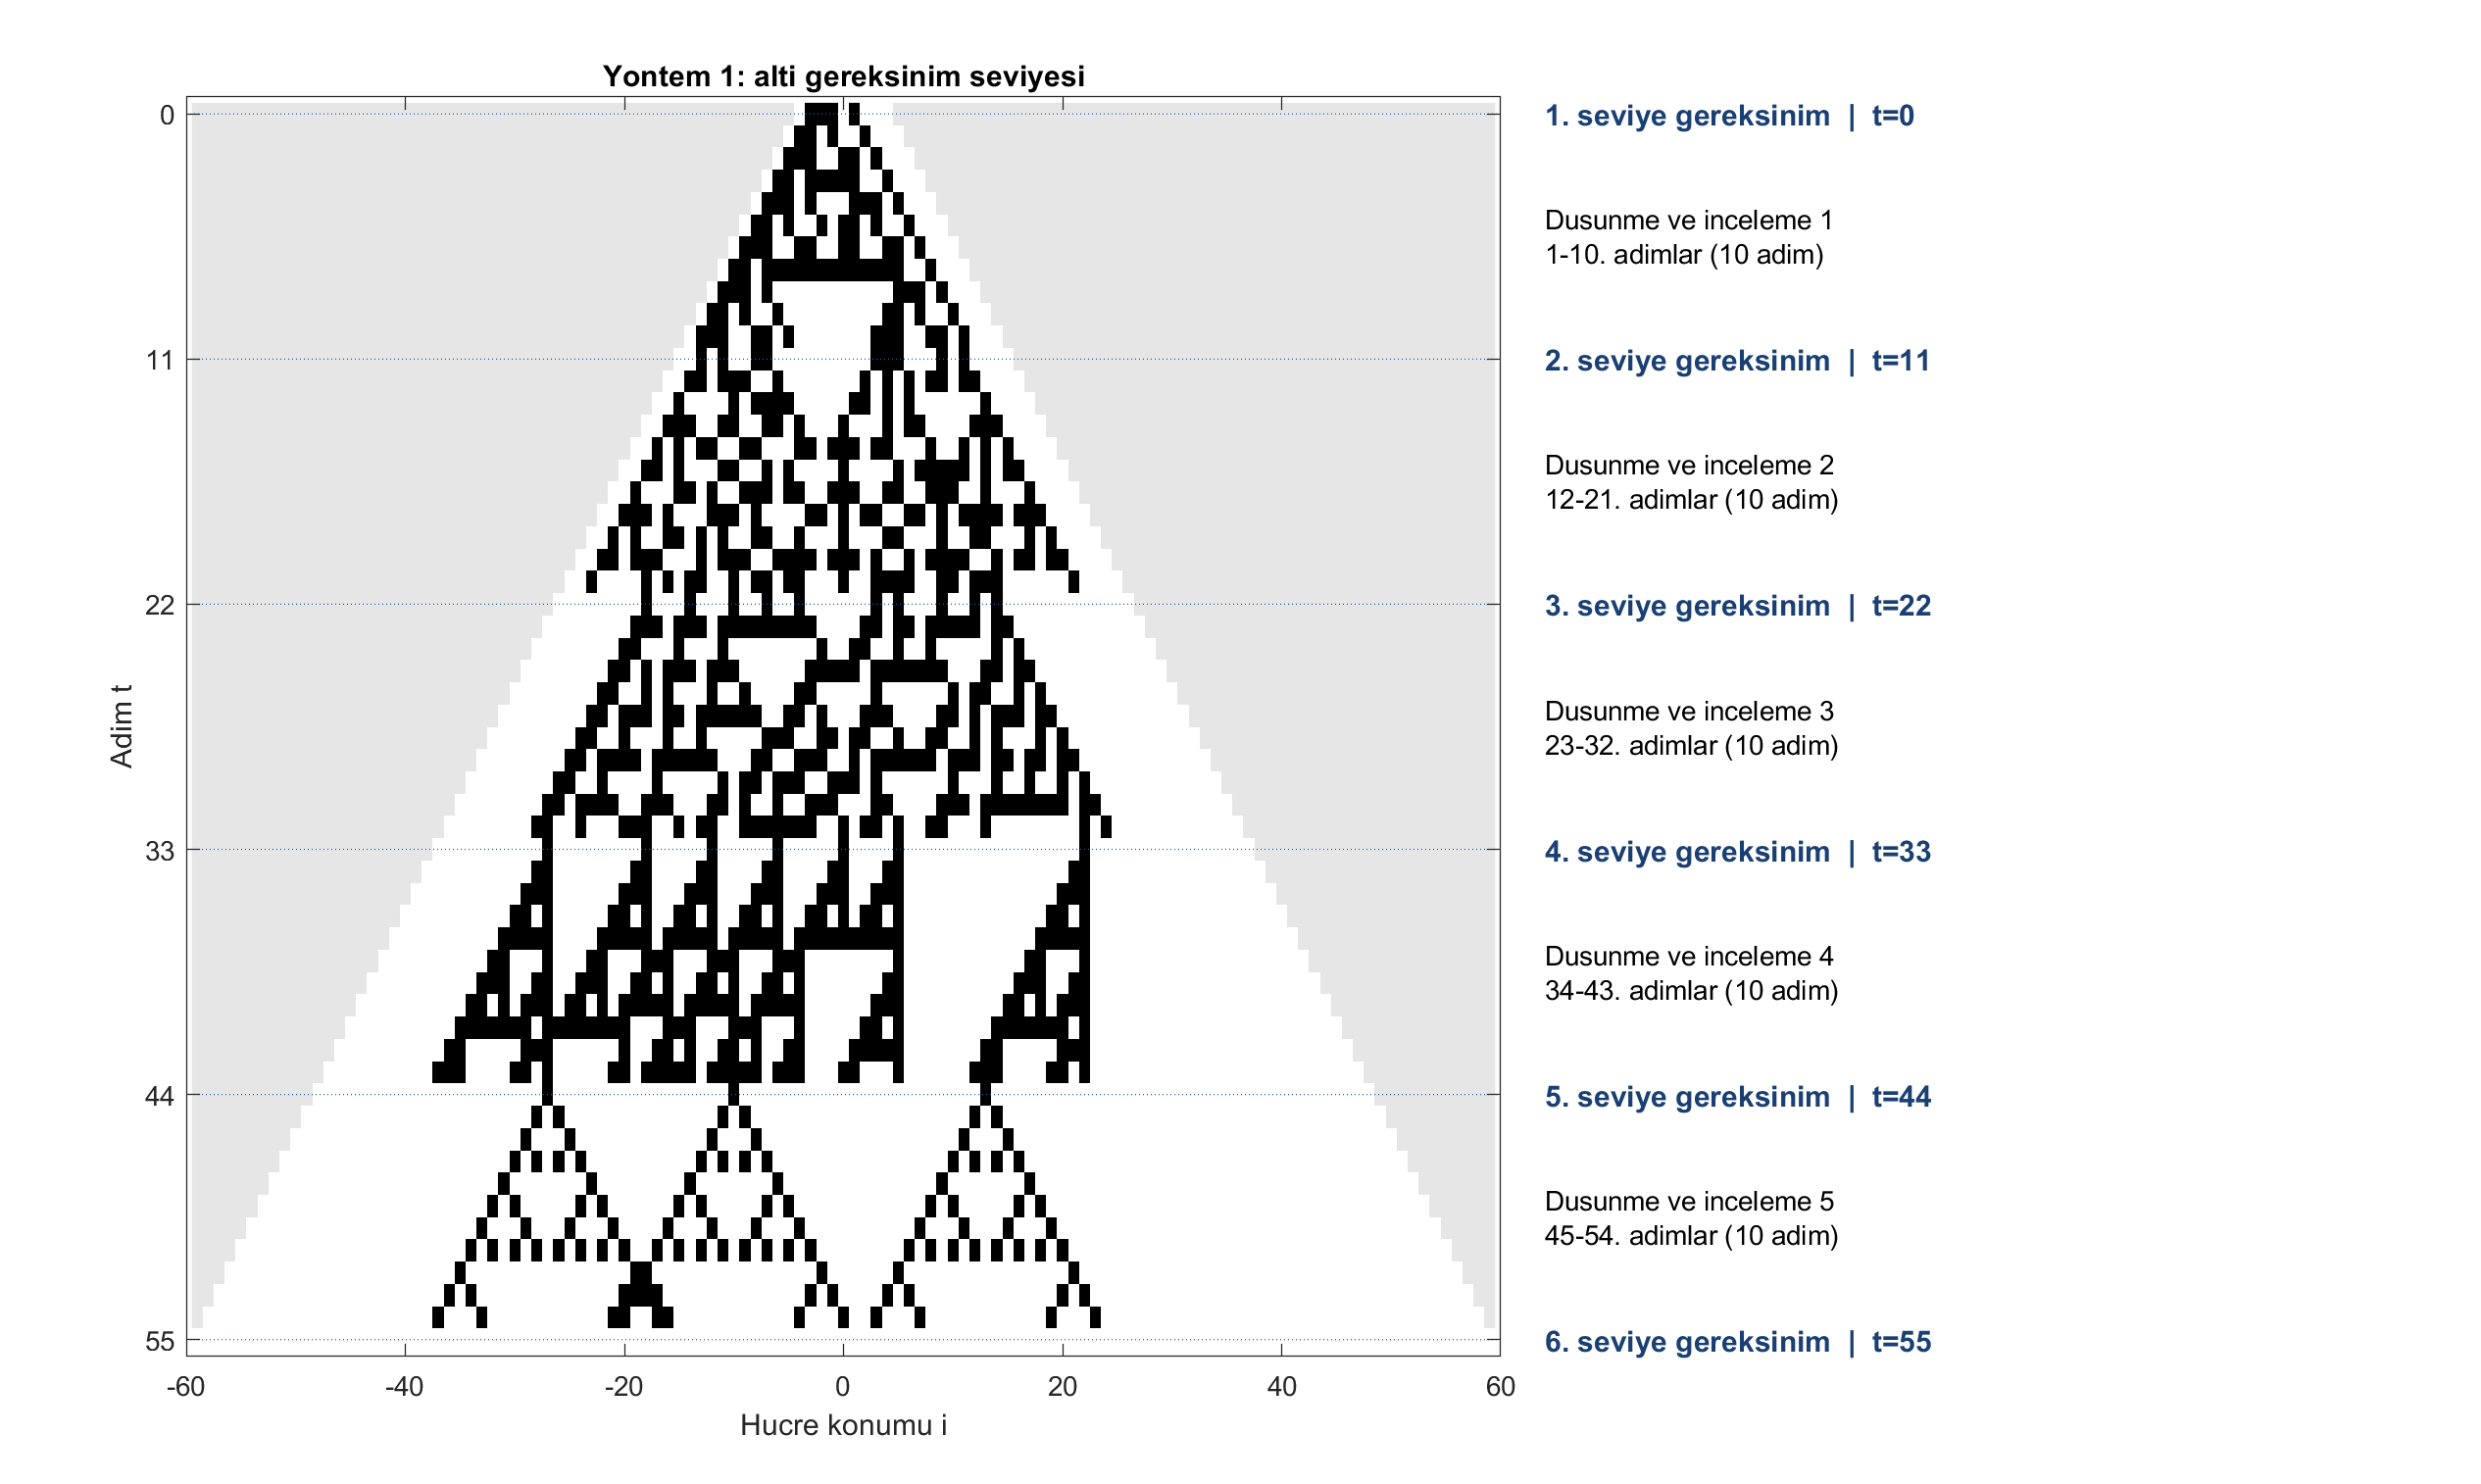
\includegraphics[width=\linewidth]{assets/image_1.png}\end{center}
\small Mavi kesikli çizgiler seviye satırlarını, sağdaki başlıklar on adımlık düşünme dönemlerini işaretler. Siyah 1, beyaz 0; gri alan ölçüm penceresi dışıdır. İşaretleme çizgileri hesaplanan hücrelere dahil değildir.\normalsize
\begin{center}\small\begin{tabular}{cr p{128mm}}\toprule Seviye & $t$ & Bu seviyede kayda geçen gereksinim kararı\\\midrule
2 & 11 & Yaş kapsamı incelenir; A=1 için ağırlık 0,8, A=0 için 0,2 olur. \\
3 & 22 & A=1 kapsamı bağlayıcı olarak seçilir; diğer üç konu açıktır. \\
4 & 33 & P0 profili seçilir: B=0. \\
5 & 44 & 10 N kuvvet hedefi seçilir: C=1. \\
6 & 55 & Tam açma-kapama seçilir: D=1; dört kabul kaydı geçer. \\
\bottomrule\end{tabular}\end{center}

\page{Yöntem 1/5 | Sayısal analiz}{Sıralı karar kapıları: entropi değişimi}
\begin{center}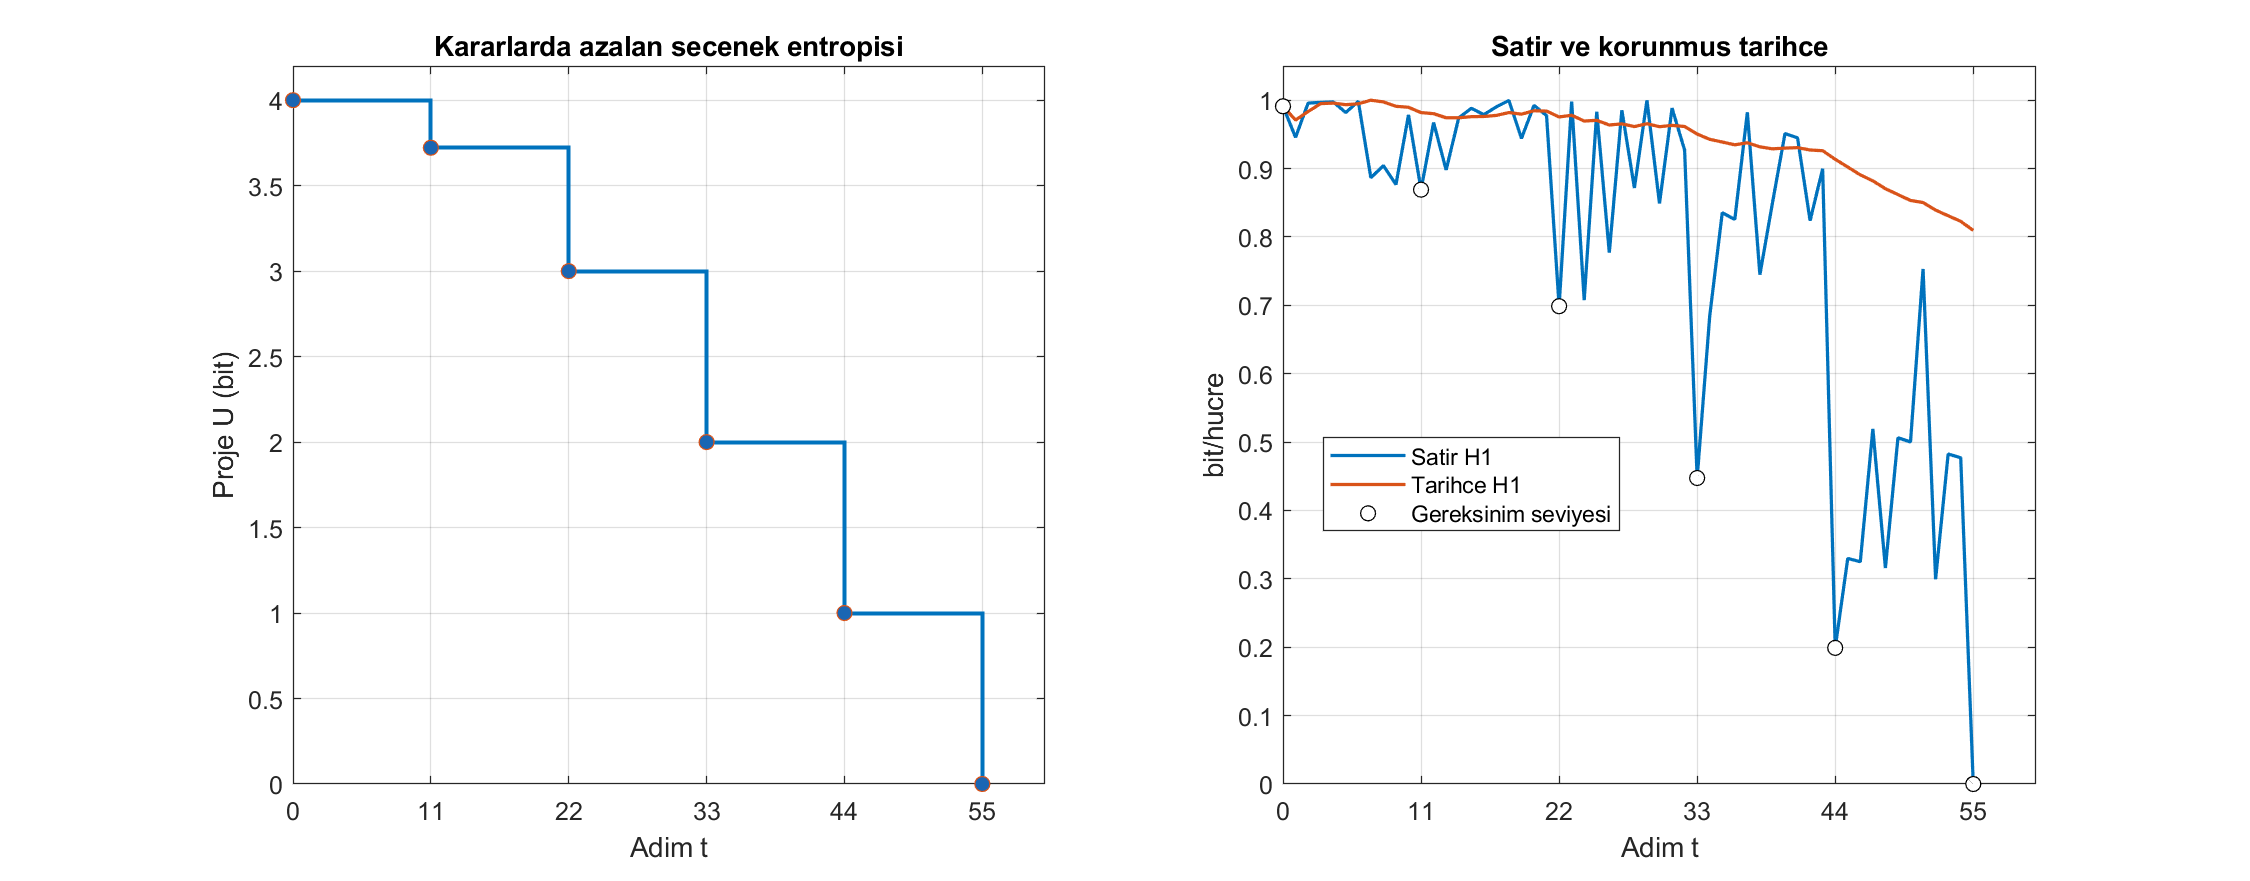
\includegraphics[width=\linewidth]{assets/entropy_1.png}\end{center}
\begin{center}\small\begin{tabular}{crrrrrr}\toprule Seviye & $t$ & Aday & Açık konu & Proje $U$ & Satır $H_1$ & Geçmiş $H_1$\\\midrule
1 & 0 & 16 & 4 & 4,0000 & 0,9911 & 0,9911 \\
2 & 11 & 16 & 4 & 3,7219 & 0,8691 & 0,9818 \\
3 & 22 & 8 & 3 & 3,0000 & 0,6987 & 0,9755 \\
4 & 33 & 4 & 2 & 2,0000 & 0,4475 & 0,9505 \\
5 & 44 & 2 & 1 & 1,0000 & 0,1990 & 0,9136 \\
6 & 55 & 1 & 0 & 0,0000 & 0,0000 & 0,8095 \\
\bottomrule\end{tabular}\end{center}
\textbf{Karar anının kontrolü.} Aynı genişlikteki geçici satır ile karar sonrası satır aşağıda karşılaştırılır. $\Delta H=H_{\rm ön}-H_{\rm son}$ pozitif olmalıdır.
\begin{center}\small\begin{tabular}{rrrrrr}\toprule $t$ & $H_{\rm ön}$ & Hedef $H^*$ & $H_{\rm son}$ & $\Delta H$ & Azalan işaret\\\midrule
11 & 0,9629 & 0,8960 & 0,8691 & 0,0938 & 3 \\
22 & 0,9687 & 0,7006 & 0,6987 & 0,2700 & 11 \\
33 & 0,9183 & 0,4658 & 0,4475 & 0,4708 & 18 \\
44 & 0,8923 & 0,2237 & 0,1990 & 0,6933 & 27 \\
55 & 0,4717 & 0,0000 & 0,0000 & 0,4717 & 12 \\
\bottomrule\end{tabular}\end{center}
\textbf{Yorum.} İlk kapı kesin eleme değil, ağırlıklandırmadır. Sonraki dört kapı sırayla A, B, C ve D konularını kapatır. Bu nedenle beş karar noktasının tamamında pozitif bir entropi azalması elde edilir. Önceki dört kapılı akışa beşinci bir kesin karar uydurmak yerine başlangıç incelemesi açıkça modellenmiştir.

İkinci seviyede $U=3+h_2(0{,}8)=3{,}7219$ bittir. Sonraki seviyeler sırasıyla 3, 2, 1 ve 0 bittir.

\page{Yöntem 2/5 | İşaretli siyah-beyaz akış}{Paralel alt çalışmalar}
\begin{center}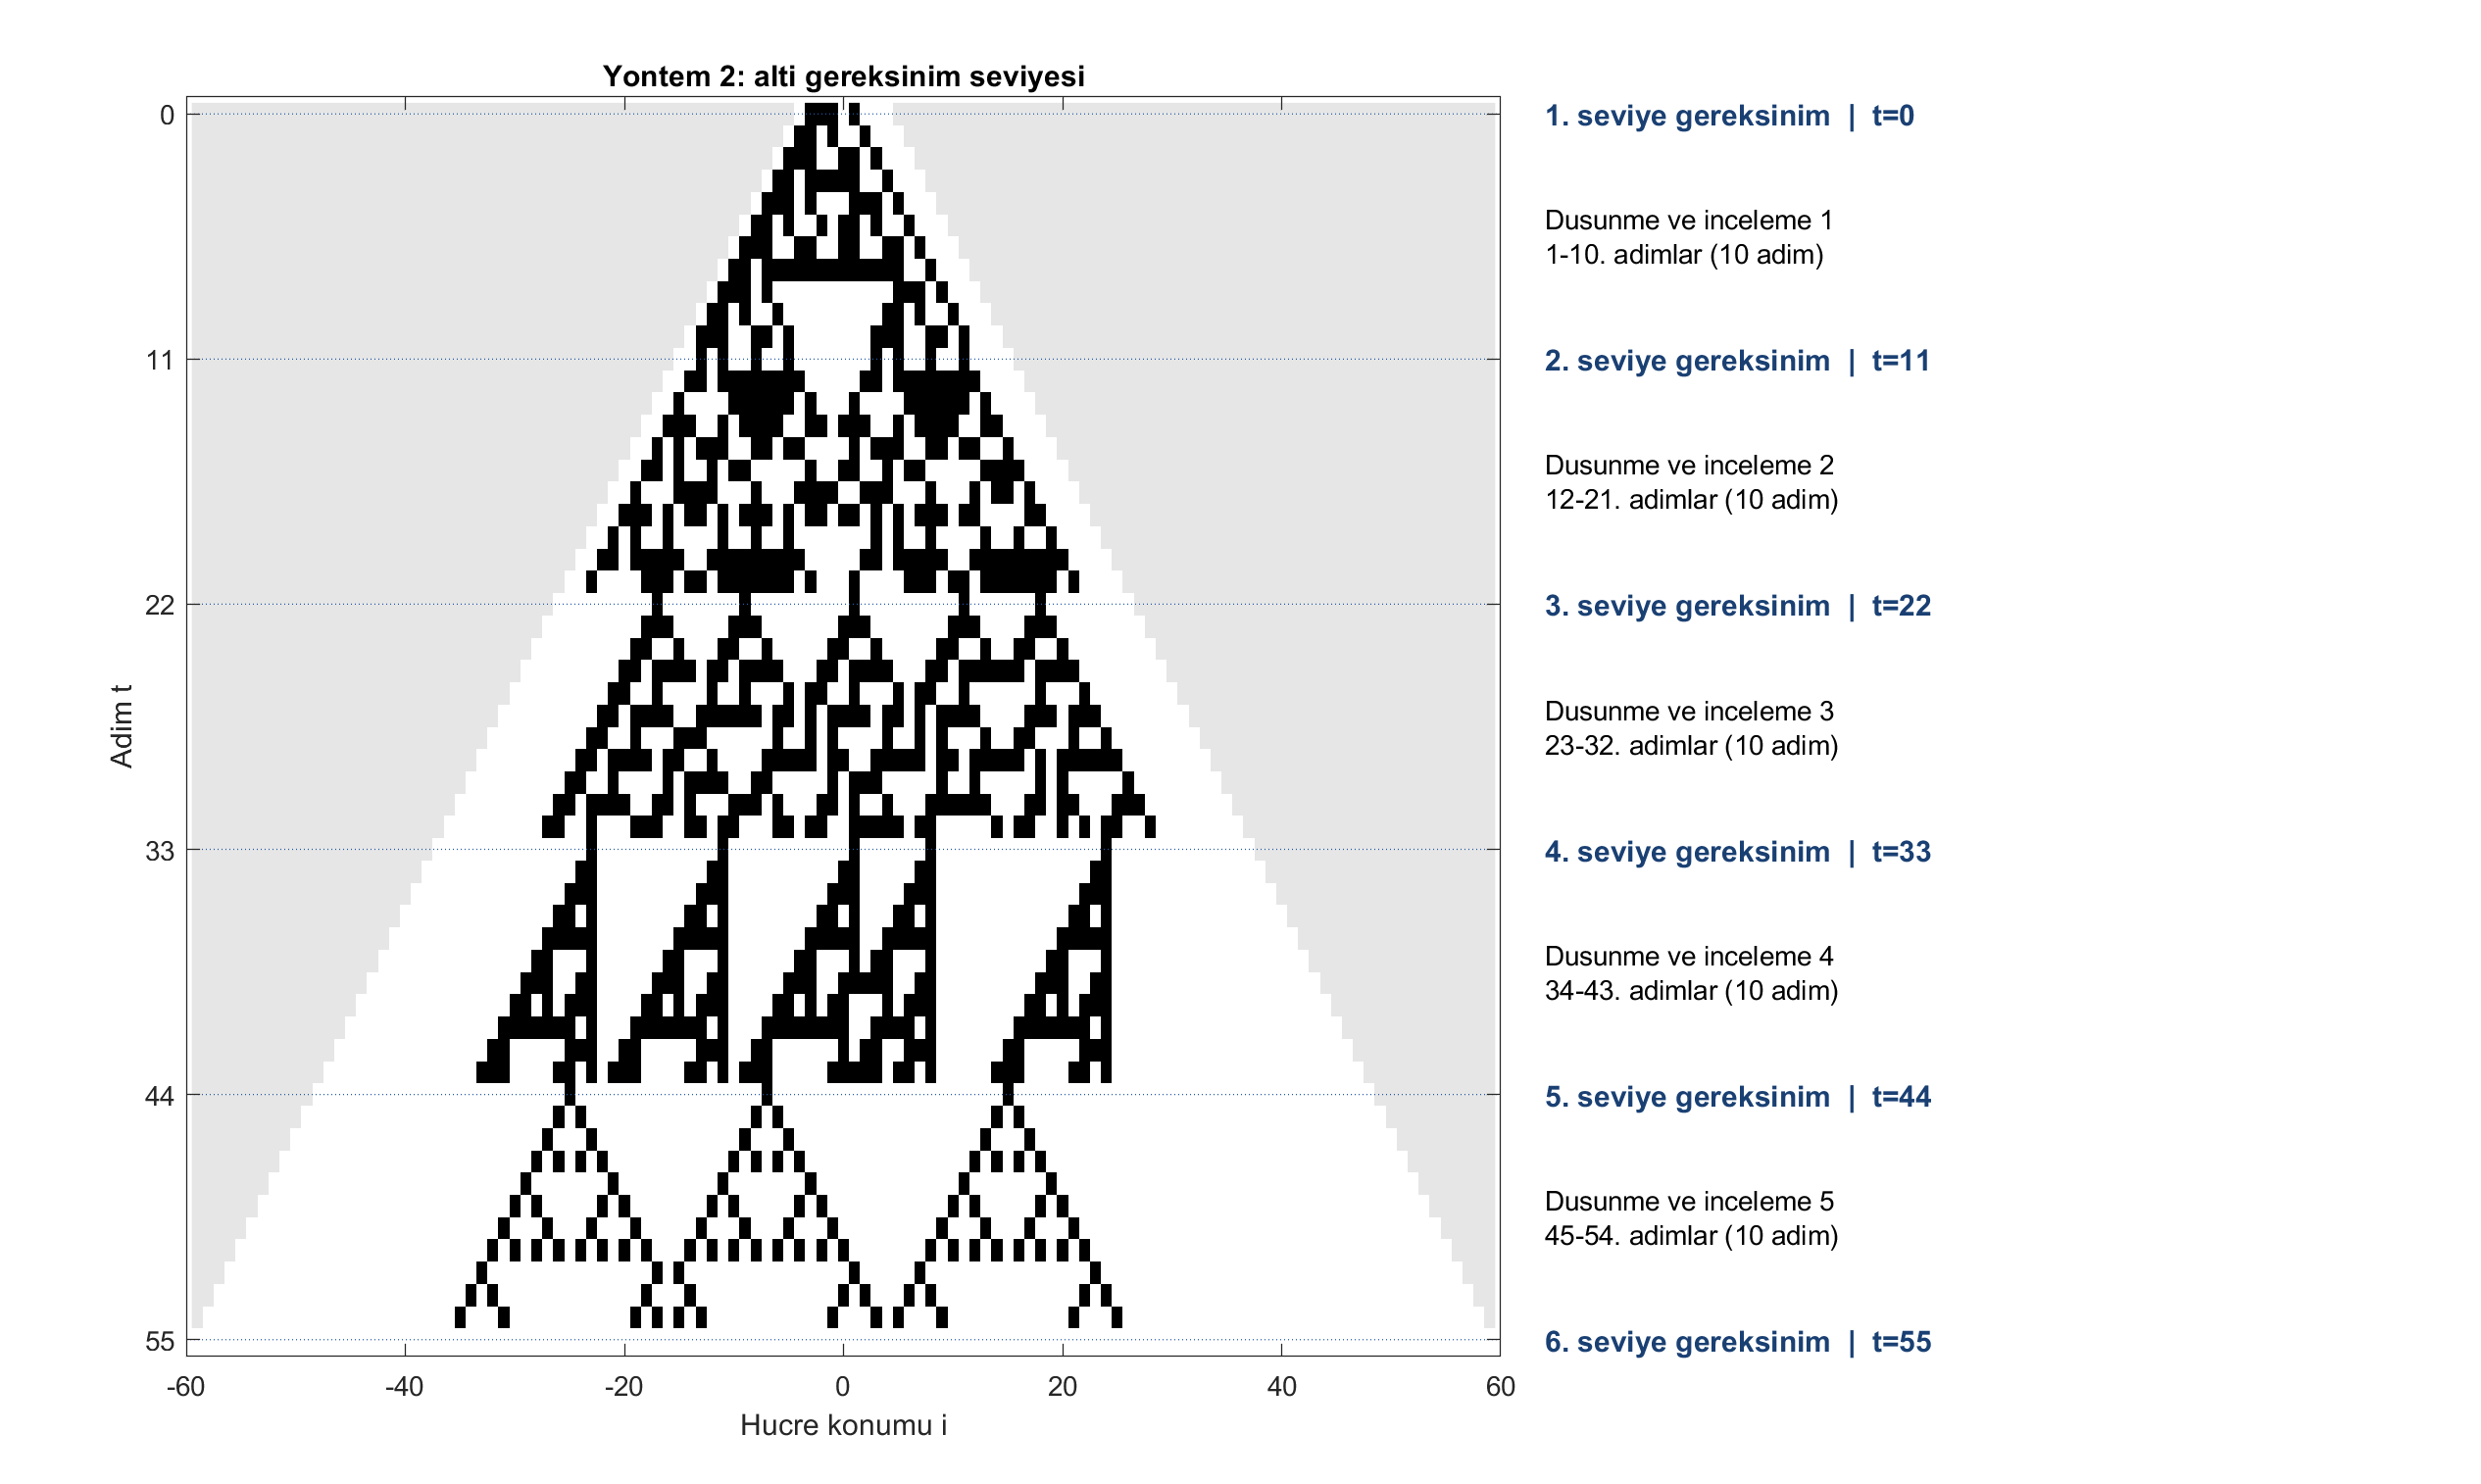
\includegraphics[width=\linewidth]{assets/image_2.png}\end{center}
\small Mavi kesikli çizgiler seviye satırlarını, sağdaki başlıklar on adımlık düşünme dönemlerini işaretler. Siyah 1, beyaz 0; gri alan ölçüm penceresi dışıdır. İşaretleme çizgileri hesaplanan hücrelere dahil değildir.\normalsize
\begin{center}\small\begin{tabular}{cr p{128mm}}\toprule Seviye & $t$ & Bu seviyede kayda geçen gereksinim kararı\\\midrule
2 & 11 & Kapsam ve profil birlikte incelenir; A=1 ve B=0 marjinalleri ayrı ayrı 0,8 olur. \\
3 & 22 & İlk iş paketi kapanır: A=1 ve B=0 birlikte seçilir. \\
4 & 33 & Mekanizma çalışması C=1 seçeneğinin ağırlığını 0,8 yapar; D açıktır. \\
5 & 44 & Kuvvet alt çalışması kapanır: C=1. \\
6 & 55 & Bütünleşik testte D=1 seçilir; dört kayıt birlikte kabul edilir. \\
\bottomrule\end{tabular}\end{center}

\page{Yöntem 2/5 | Sayısal analiz}{Paralel alt çalışmalar: entropi değişimi}
\begin{center}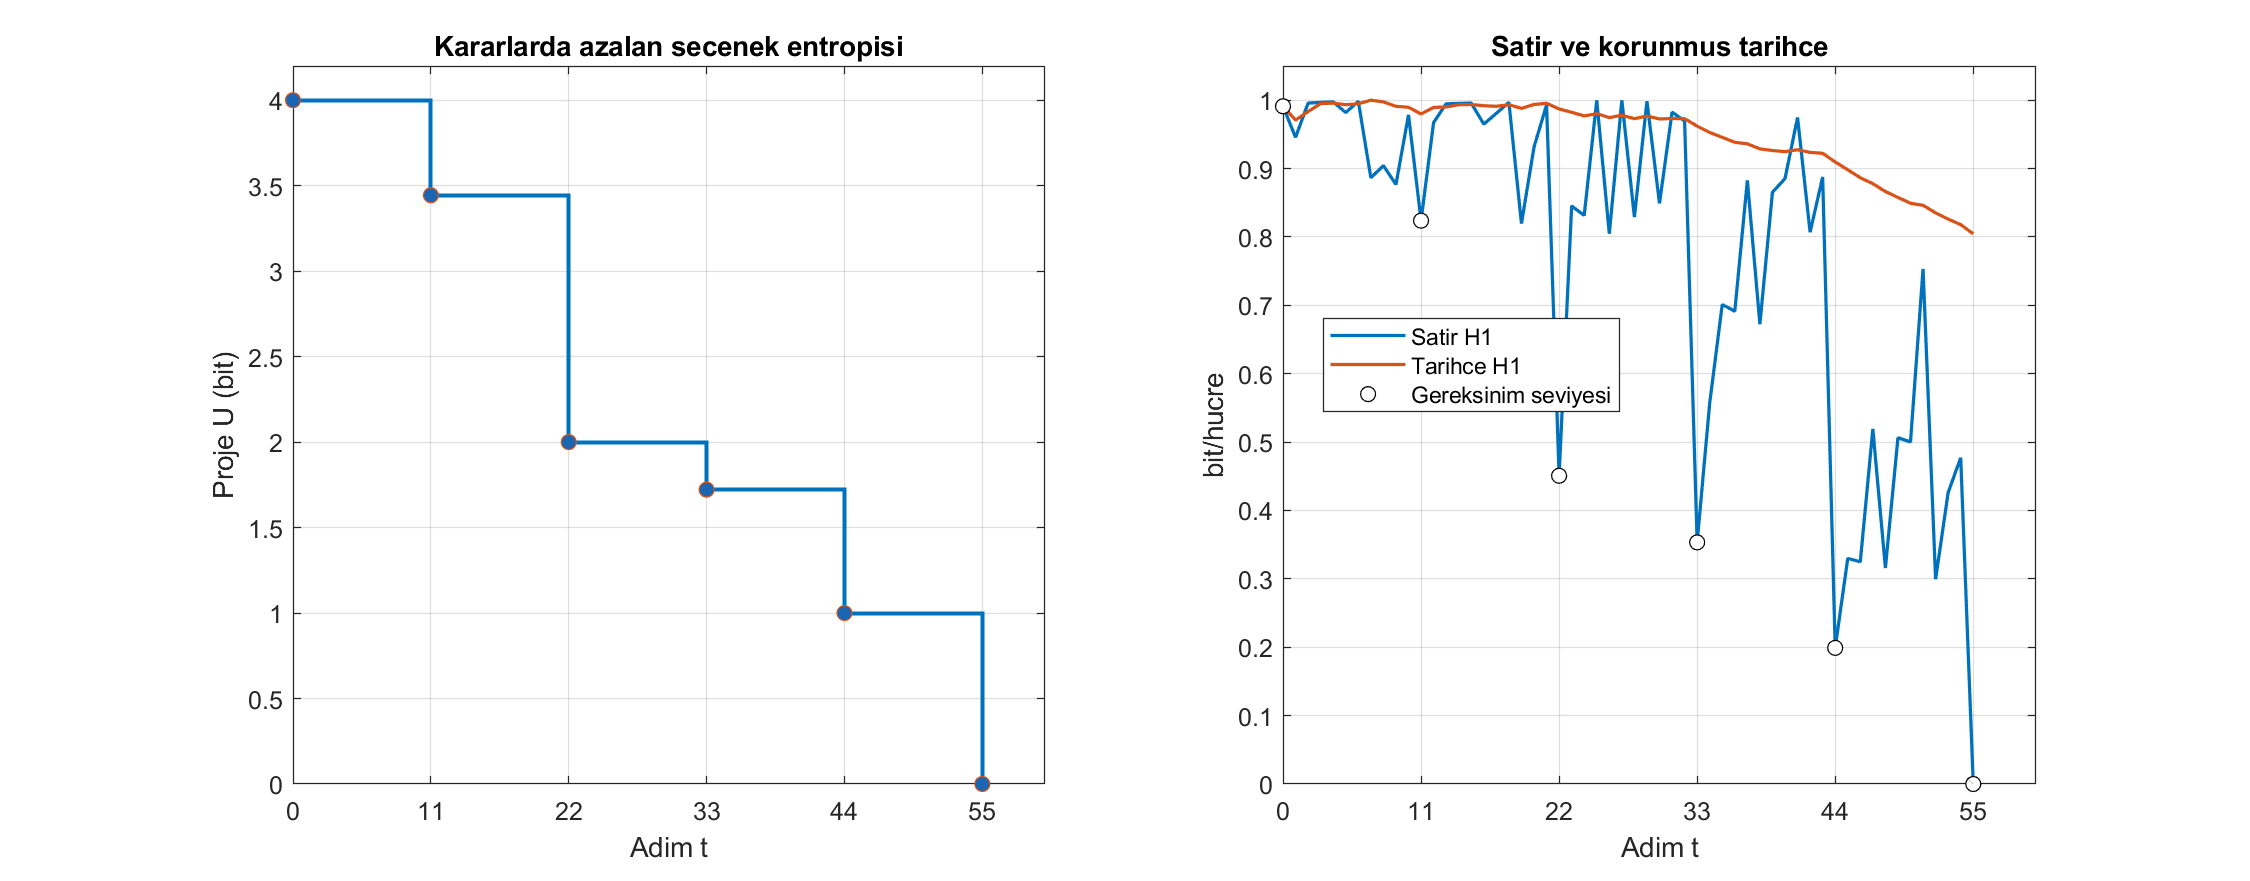
\includegraphics[width=\linewidth]{assets/entropy_2.png}\end{center}
\begin{center}\small\begin{tabular}{crrrrrr}\toprule Seviye & $t$ & Aday & Açık konu & Proje $U$ & Satır $H_1$ & Geçmiş $H_1$\\\midrule
1 & 0 & 16 & 4 & 4,0000 & 0,9911 & 0,9911 \\
2 & 11 & 16 & 4 & 3,4439 & 0,8238 & 0,9799 \\
3 & 22 & 4 & 2 & 2,0000 & 0,4508 & 0,9872 \\
4 & 33 & 4 & 2 & 1,7219 & 0,3534 & 0,9621 \\
5 & 44 & 2 & 1 & 1,0000 & 0,1990 & 0,9097 \\
6 & 55 & 1 & 0 & 0,0000 & 0,0000 & 0,8046 \\
\bottomrule\end{tabular}\end{center}
\textbf{Karar anının kontrolü.} Aynı genişlikteki geçici satır ile karar sonrası satır aşağıda karşılaştırılır. $\Delta H=H_{\rm ön}-H_{\rm son}$ pozitif olmalıdır.
\begin{center}\small\begin{tabular}{rrrrrr}\toprule $t$ & $H_{\rm ön}$ & Hedef $H^*$ & $H_{\rm son}$ & $\Delta H$ & Azalan işaret\\\midrule
11 & 0,9629 & 0,8290 & 0,8238 & 0,1391 & 4 \\
22 & 0,9977 & 0,4784 & 0,4508 & 0,5469 & 23 \\
33 & 0,9626 & 0,3881 & 0,3534 & 0,6093 & 24 \\
44 & 0,8800 & 0,2052 & 0,1990 & 0,6810 & 26 \\
55 & 0,4717 & 0,0000 & 0,0000 & 0,4717 & 12 \\
\bottomrule\end{tabular}\end{center}
\textbf{Yorum.} Birinci iş paketi kullanıcı kapsamı ve profili; ikinci paket mekanizma ve işlev üzerinde çalışır. İlk kapıda iki konu birlikte güncellenir; ikinci kapıda birlikte sabitlenir. Ayrı paketler kapansa da son gereksinim seviyesi ancak bütünleşik kabulden sonra tamamlanır.

İkinci seviyede $U=2+2h_2(0{,}8)=3{,}4439$; dördüncü seviyede $U=1+h_2(0{,}8)=1{,}7219$ bittir.

\page{Yöntem 3/5 | İşaretli siyah-beyaz akış}{Kısıtlarla seçenek daraltma}
\begin{center}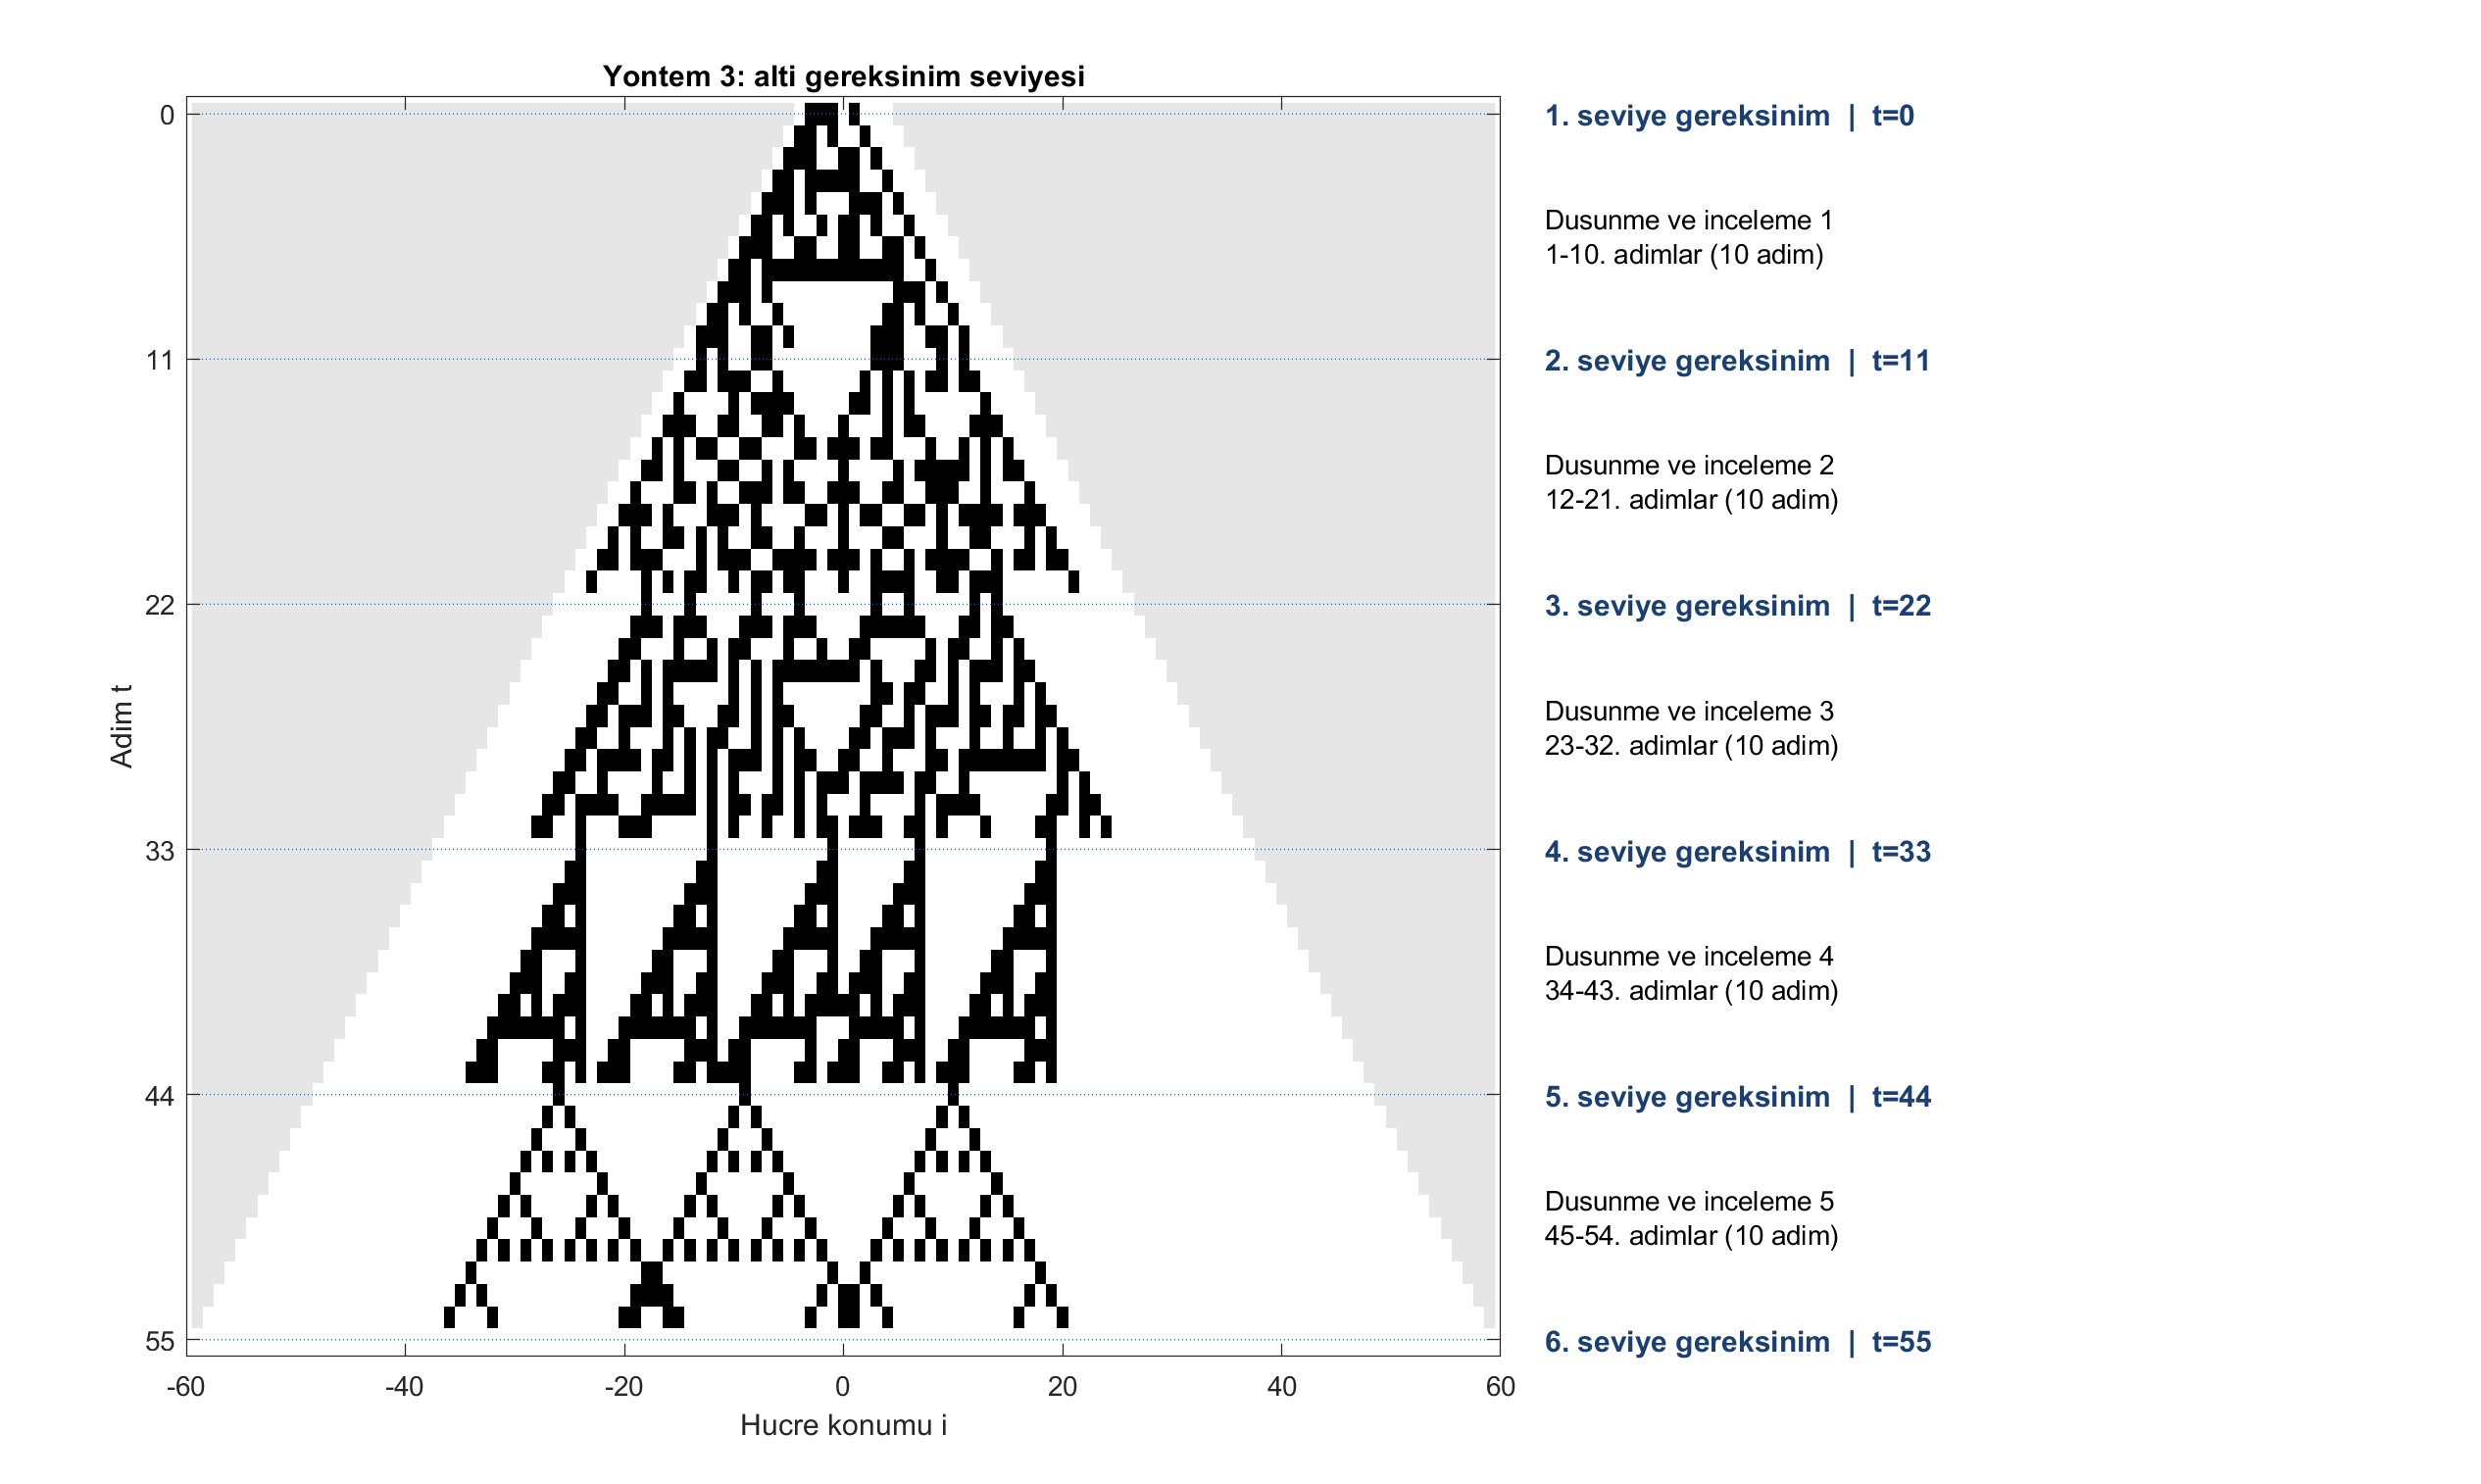
\includegraphics[width=\linewidth]{assets/image_3.png}\end{center}
\small Mavi kesikli çizgiler seviye satırlarını, sağdaki başlıklar on adımlık düşünme dönemlerini işaretler. Siyah 1, beyaz 0; gri alan ölçüm penceresi dışıdır. İşaretleme çizgileri hesaplanan hücrelere dahil değildir.\normalsize
\begin{center}\small\begin{tabular}{cr p{128mm}}\toprule Seviye & $t$ & Bu seviyede kayda geçen gereksinim kararı\\\midrule
2 & 11 & Kapsam incelemesi A=1 seçeneğine 0,8 ağırlık verir. \\
3 & 22 & Paket politikası B=1-A kabul edilir; uygun olmayan paketler çıkarılır. \\
4 & 33 & İkinci bağlantı C=A kabul edilir; adaylar yeniden daralır. \\
5 & 44 & A=1 seçilir; bağlantılar B=0 ve C=1 sonucunu verir. \\
6 & 55 & D=1 seçilir; bağlantılar ve ürün kabul kayıtları doğrulanır. \\
\bottomrule\end{tabular}\end{center}

\page{Yöntem 3/5 | Sayısal analiz}{Kısıtlarla seçenek daraltma: entropi değişimi}
\begin{center}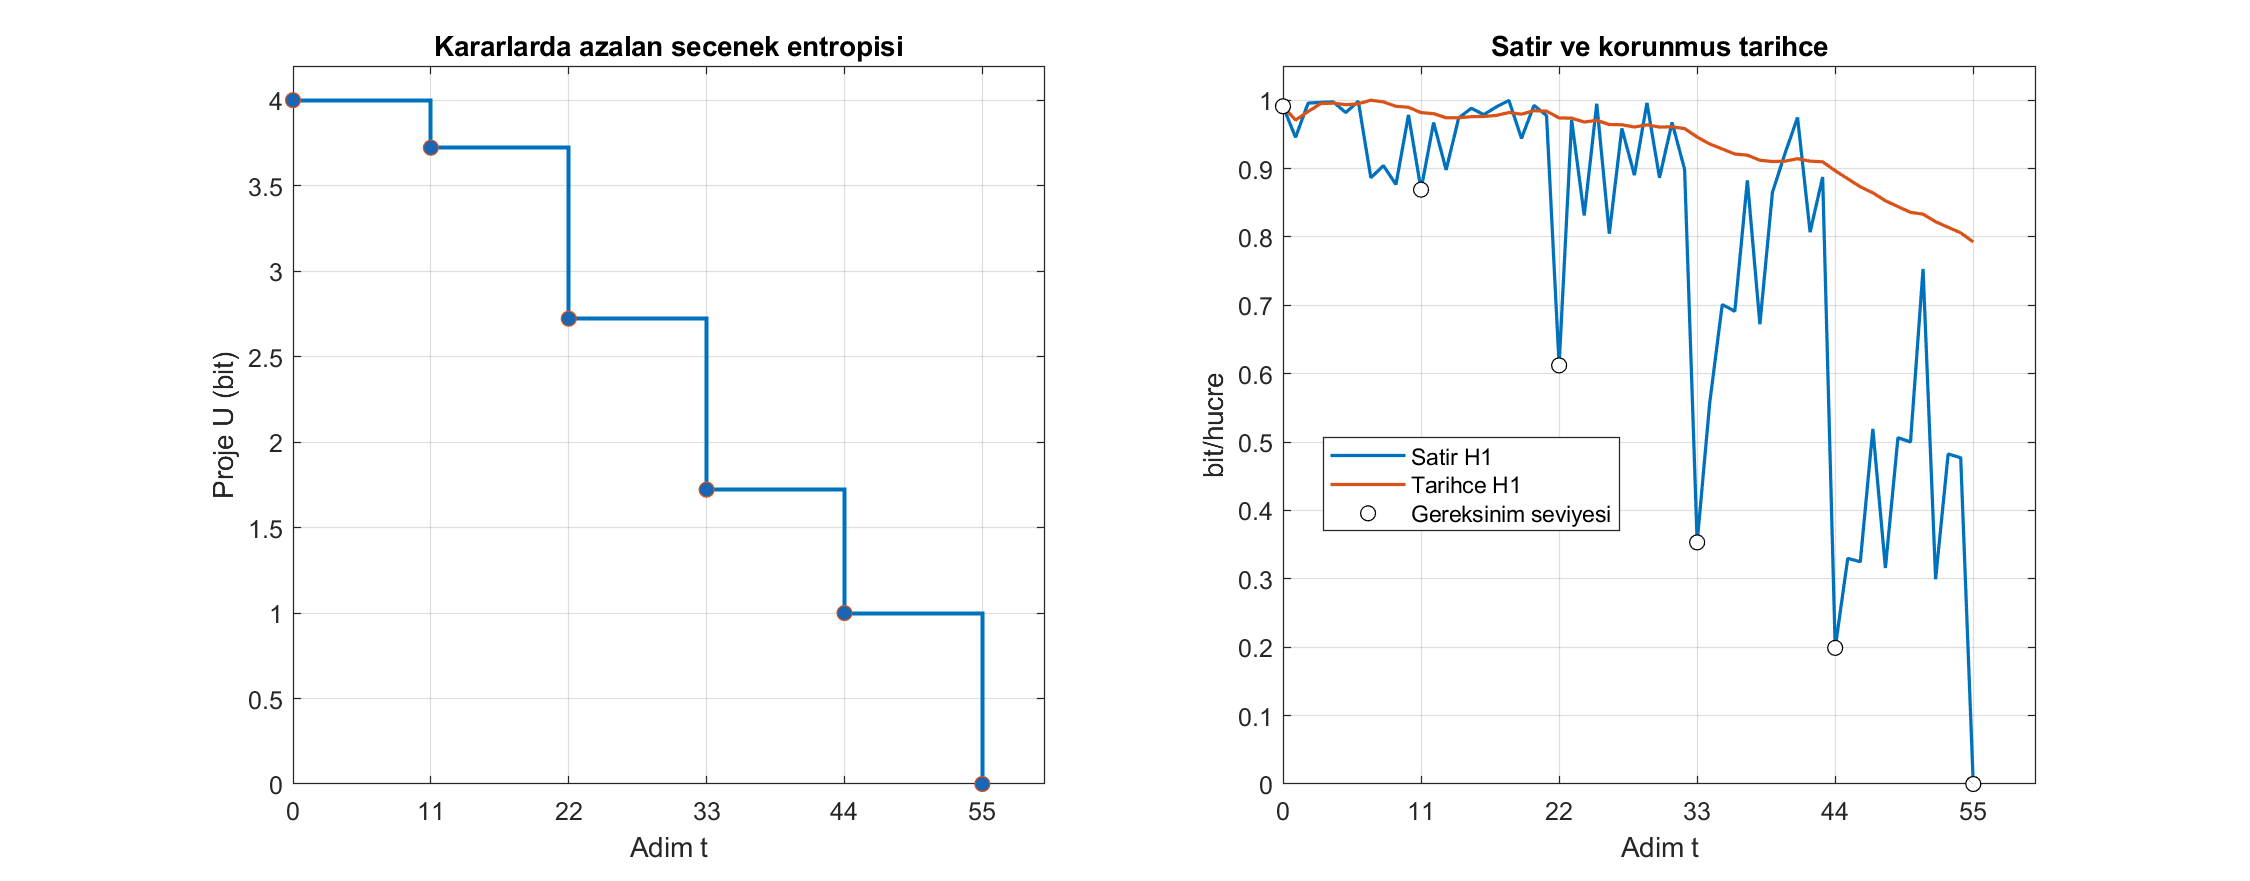
\includegraphics[width=\linewidth]{assets/entropy_3.png}\end{center}
\begin{center}\small\begin{tabular}{crrrrrr}\toprule Seviye & $t$ & Aday & Açık konu & Proje $U$ & Satır $H_1$ & Geçmiş $H_1$\\\midrule
1 & 0 & 16 & 4 & 4,0000 & 0,9911 & 0,9911 \\
2 & 11 & 16 & 4 & 3,7219 & 0,8691 & 0,9818 \\
3 & 22 & 8 & 4 & 2,7219 & 0,6122 & 0,9740 \\
4 & 33 & 4 & 4 & 1,7219 & 0,3534 & 0,9461 \\
5 & 44 & 2 & 1 & 1,0000 & 0,1990 & 0,8968 \\
6 & 55 & 1 & 0 & 0,0000 & 0,0000 & 0,7926 \\
\bottomrule\end{tabular}\end{center}
\textbf{Karar anının kontrolü.} Aynı genişlikteki geçici satır ile karar sonrası satır aşağıda karşılaştırılır. $\Delta H=H_{\rm ön}-H_{\rm son}$ pozitif olmalıdır.
\begin{center}\small\begin{tabular}{rrrrrr}\toprule $t$ & $H_{\rm ön}$ & Hedef $H^*$ & $H_{\rm son}$ & $\Delta H$ & Azalan işaret\\\midrule
11 & 0,9629 & 0,8960 & 0,8691 & 0,0938 & 3 \\
22 & 0,9687 & 0,6356 & 0,6122 & 0,3565 & 13 \\
33 & 0,8893 & 0,3873 & 0,3534 & 0,5359 & 18 \\
44 & 0,8800 & 0,2052 & 0,1990 & 0,6810 & 26 \\
55 & 0,4717 & 0,0000 & 0,0000 & 0,4717 & 12 \\
\bottomrule\end{tabular}\end{center}
\textbf{Yorum.} Aynı aday kümesinde bağımlılık eklemek de belirsizliği azaltabilir. B=1-A ve C=A, bu örneğe özgü paket politikalarıdır; yaş veya kuvvet hakkında fizik yasası değildir. Bağlantılar yanlışsa sonucun kesin görünmesi yeterli olmaz; politikalar ve fiziksel tasarım ayrı doğrulanmalıdır.

Bağlantılar eklendiğinde bağımsız seçenek boyutu azalır. İkinci, üçüncü ve dördüncü seviyeler $3+h_2(0{,}8)$, $2+h_2(0{,}8)$ ve $1+h_2(0{,}8)$ bittir.

\page{Yöntem 4/5 | İşaretli siyah-beyaz akış}{Kanıt güncellemesi ve kesin kabul}
\begin{center}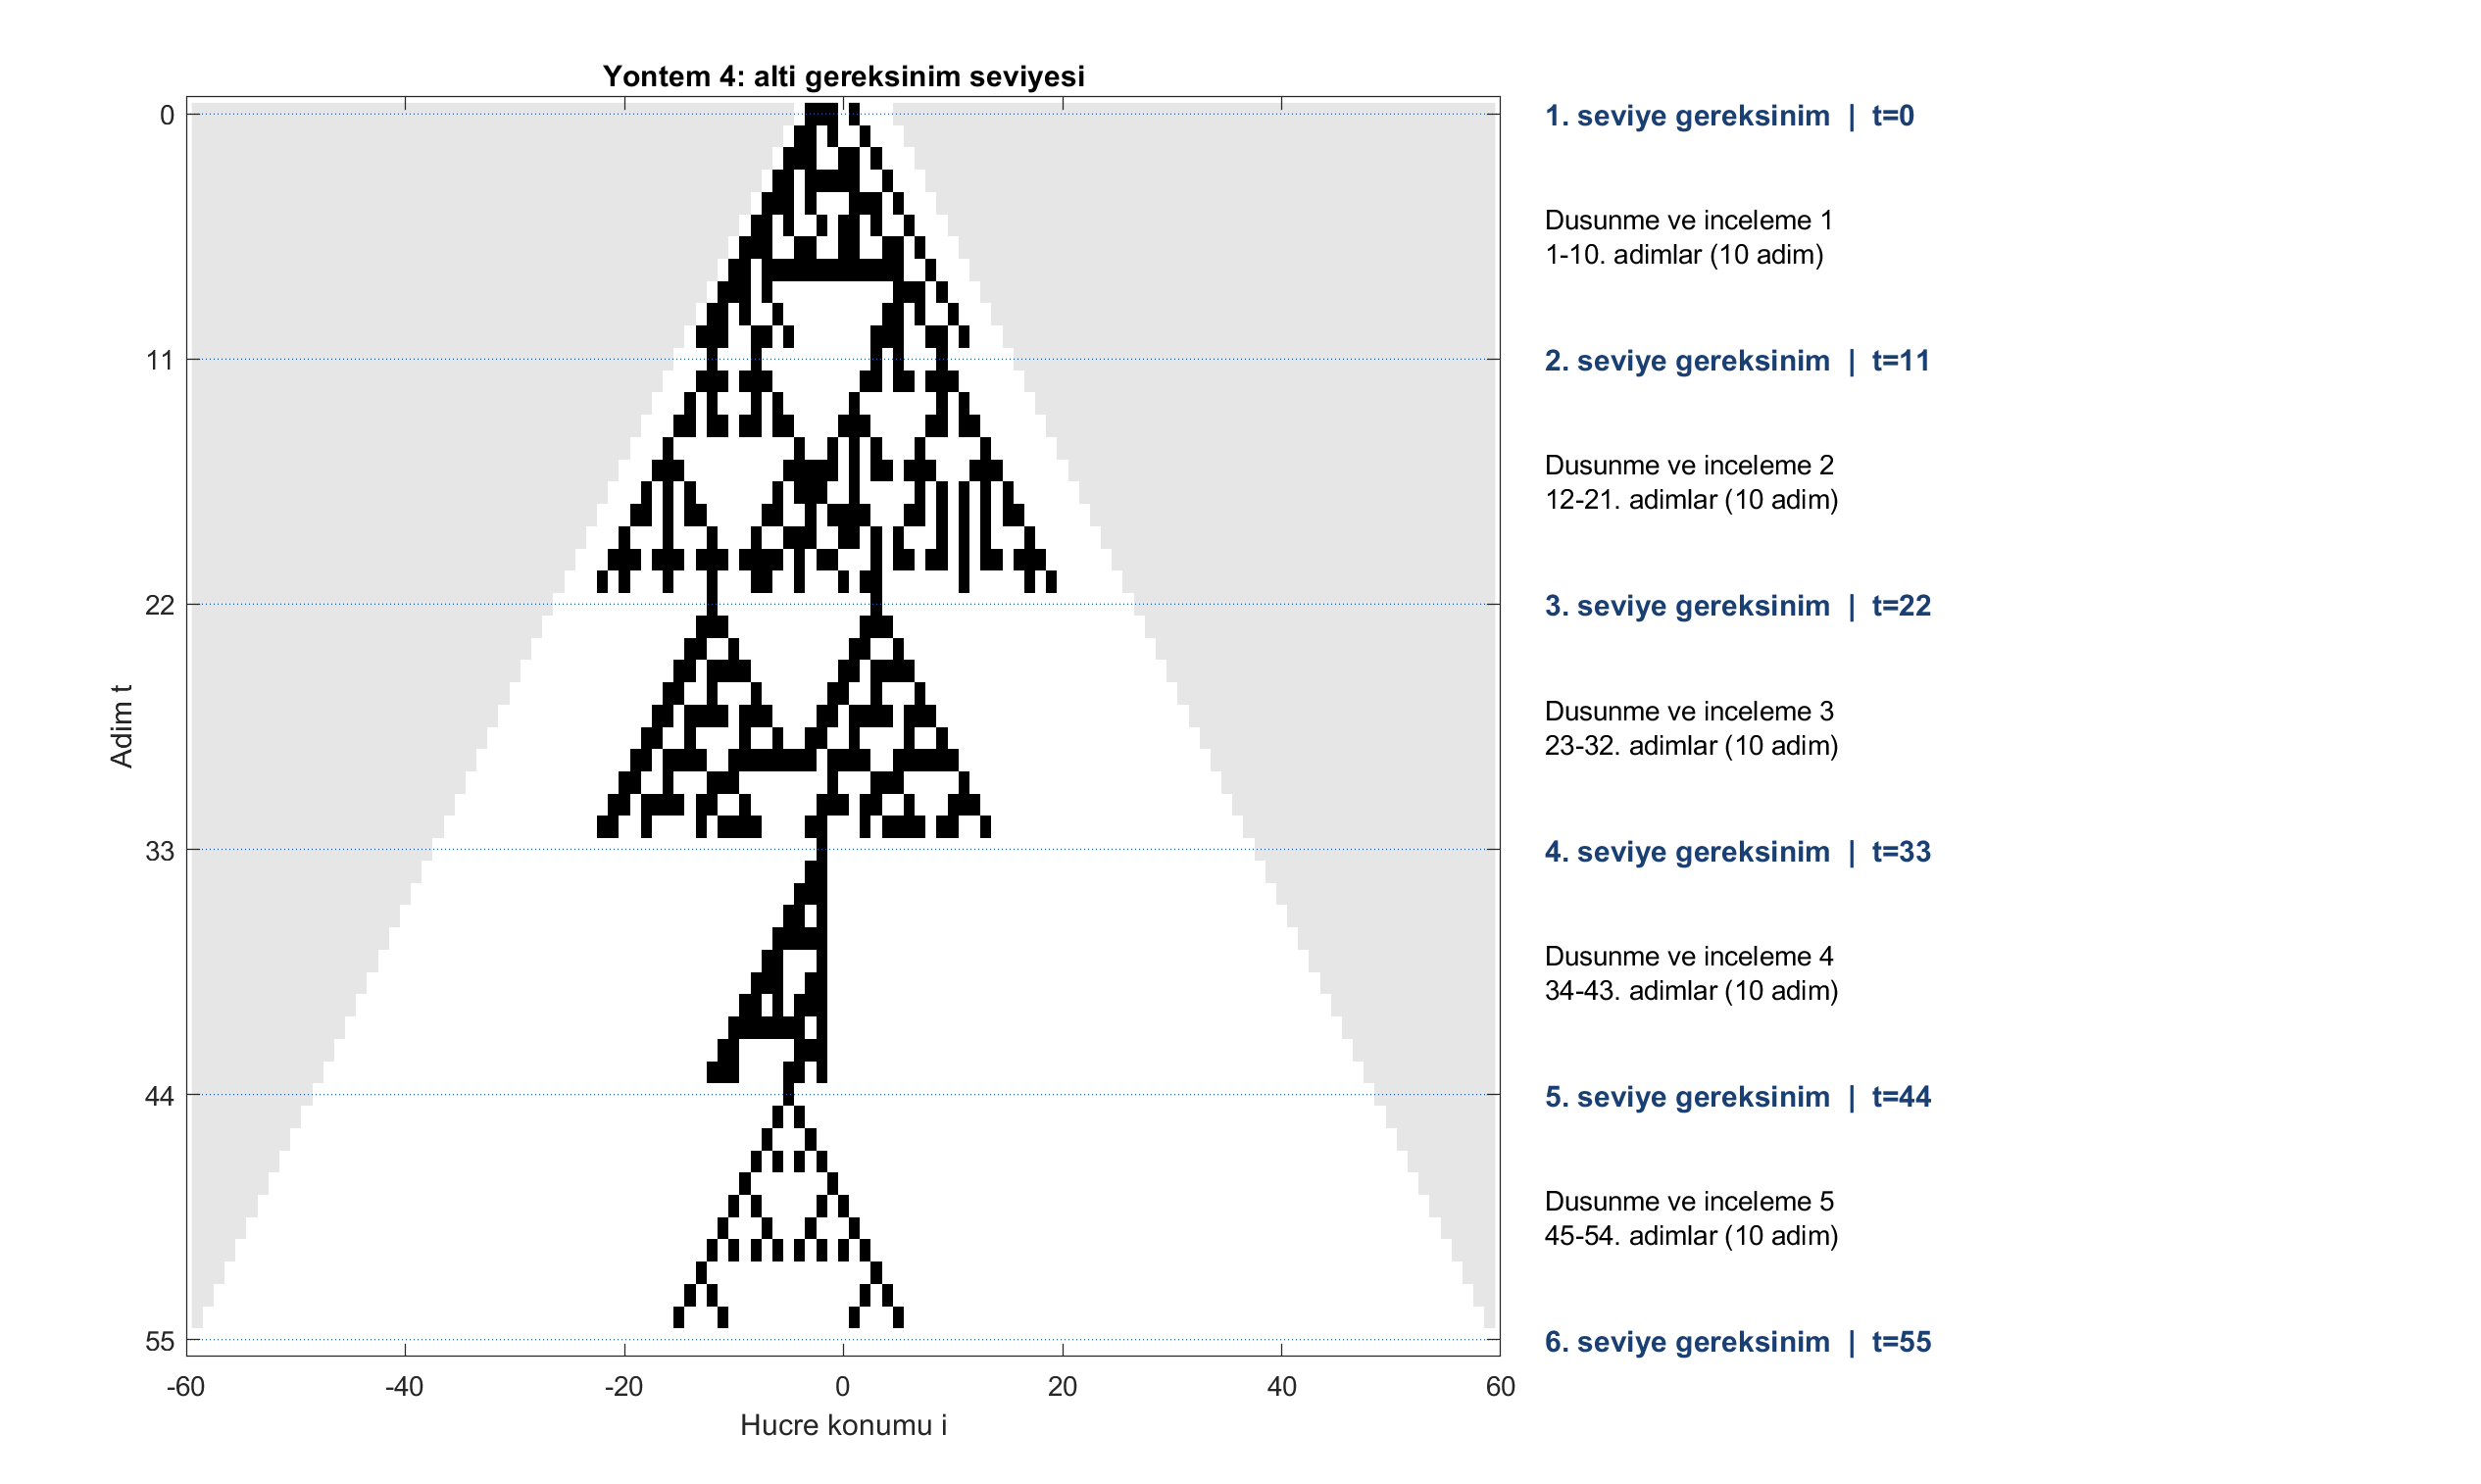
\includegraphics[width=\linewidth]{assets/image_4.png}\end{center}
\small Mavi kesikli çizgiler seviye satırlarını, sağdaki başlıklar on adımlık düşünme dönemlerini işaretler. Siyah 1, beyaz 0; gri alan ölçüm penceresi dışıdır. İşaretleme çizgileri hesaplanan hücrelere dahil değildir.\normalsize
\begin{center}\small\begin{tabular}{cr p{128mm}}\toprule Seviye & $t$ & Bu seviyede kayda geçen gereksinim kararı\\\midrule
2 & 11 & Birinci kanıt: her konu için hedef seçeneğe 4:1 olabilirlik oranı. \\
3 & 22 & İkinci bağımsız kanıt ile aynı güncelleme tekrarlanır. \\
4 & 33 & Üçüncü bağımsız kanıt eklenir; tüm adaylar hâlâ pozitiftir. \\
5 & 44 & Dördüncü bağımsız kanıt eklenir; güven artar, tam kesinlik oluşmaz. \\
6 & 55 & Bağlayıcı 1011 seçimi ve başarılı kabul kaydıyla kapsam kapatılır. \\
\bottomrule\end{tabular}\end{center}

\page{Yöntem 4/5 | Sayısal analiz}{Kanıt güncellemesi ve kesin kabul: entropi değişimi}
\begin{center}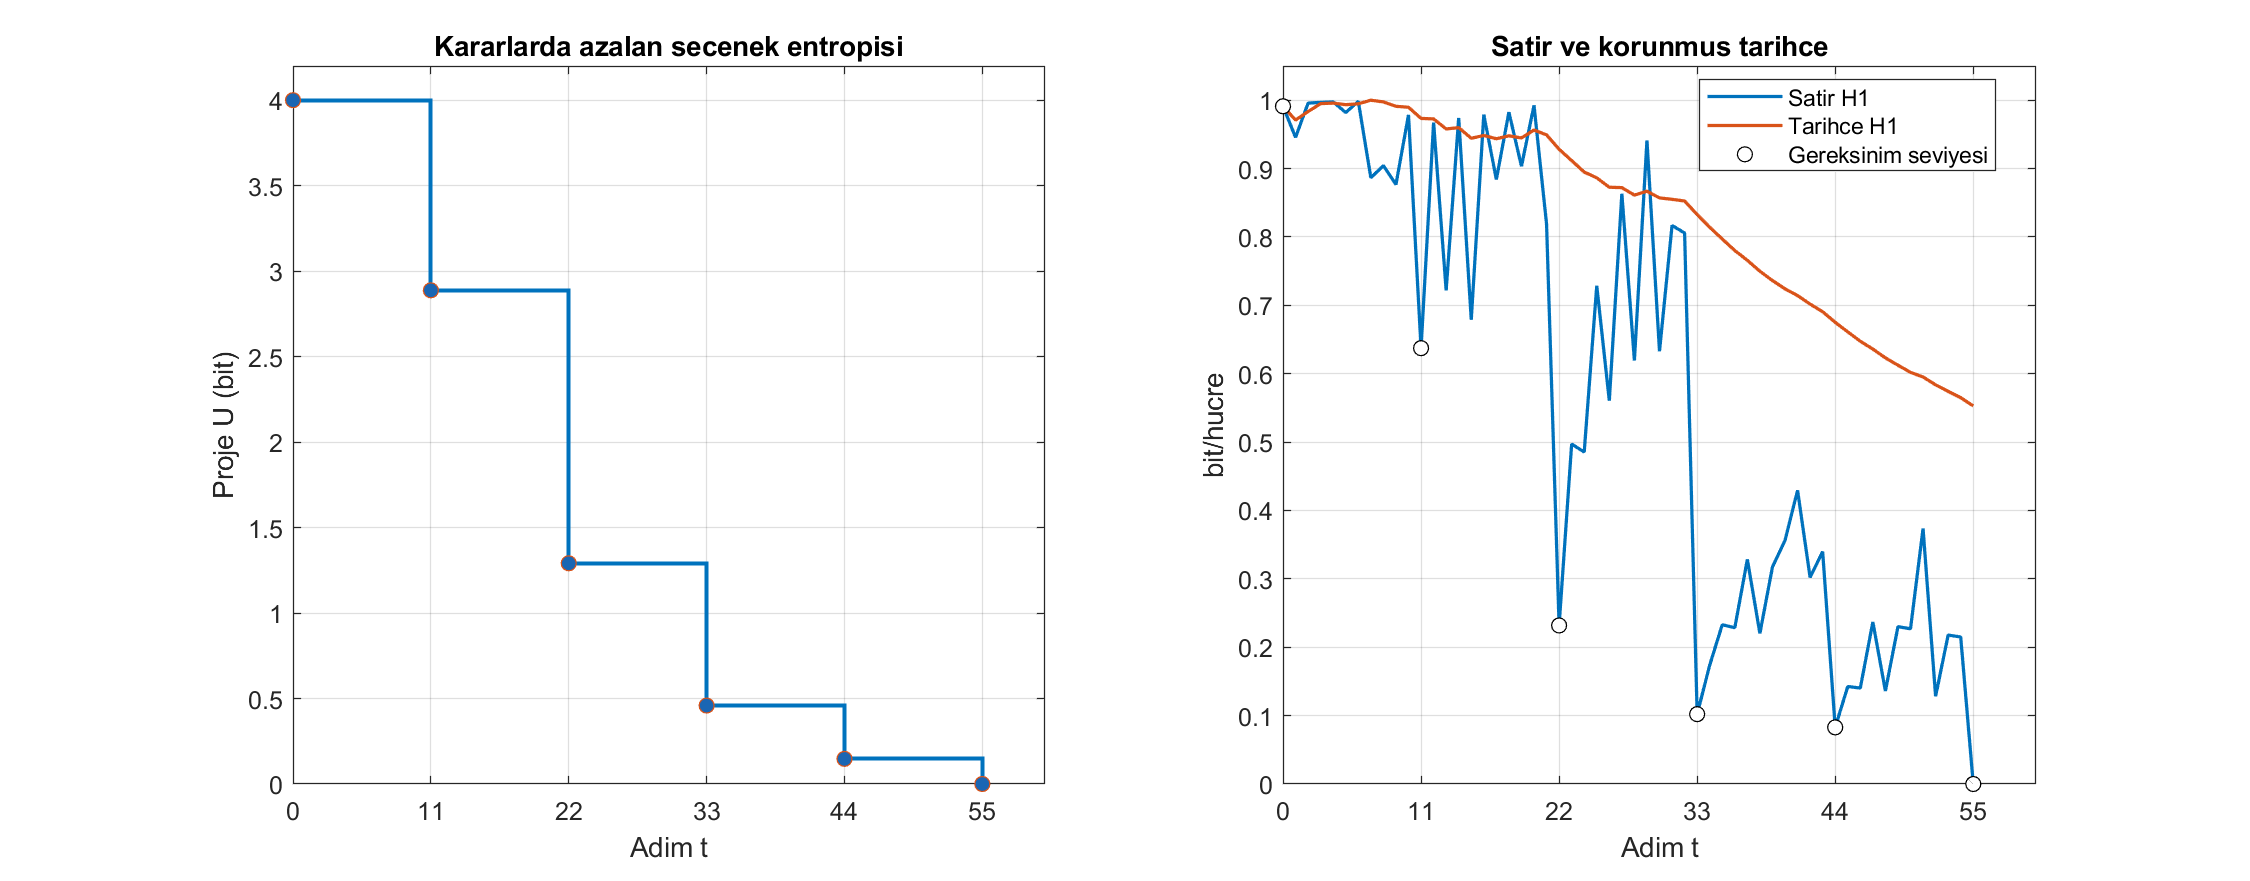
\includegraphics[width=\linewidth]{assets/entropy_4.png}\end{center}
\begin{center}\small\begin{tabular}{crrrrrr}\toprule Seviye & $t$ & Aday & Açık konu & Proje $U$ & Satır $H_1$ & Geçmiş $H_1$\\\midrule
1 & 0 & 16 & 4 & 4,0000 & 0,9911 & 0,9911 \\
2 & 11 & 16 & 4 & 2,8877 & 0,6374 & 0,9733 \\
3 & 22 & 16 & 4 & 1,2910 & 0,2318 & 0,9282 \\
4 & 33 & 16 & 4 & 0,4587 & 0,1022 & 0,8327 \\
5 & 44 & 16 & 4 & 0,1470 & 0,0828 & 0,6752 \\
6 & 55 & 1 & 0 & 0,0000 & 0,0000 & 0,5529 \\
\bottomrule\end{tabular}\end{center}
\textbf{Karar anının kontrolü.} Aynı genişlikteki geçici satır ile karar sonrası satır aşağıda karşılaştırılır. $\Delta H=H_{\rm ön}-H_{\rm son}$ pozitif olmalıdır.
\begin{center}\small\begin{tabular}{rrrrrr}\toprule $t$ & $H_{\rm ön}$ & Hedef $H^*$ & $H_{\rm son}$ & $\Delta H$ & Azalan işaret\\\midrule
11 & 0,9629 & 0,6951 & 0,6374 & 0,3255 & 7 \\
22 & 0,8037 & 0,2850 & 0,2318 & 0,5719 & 11 \\
33 & 0,7950 & 0,0824 & 0,1022 & 0,6929 & 17 \\
44 & 0,3348 & 0,0327 & 0,0828 & 0,2519 & 5 \\
55 & 0,2122 & 0,0000 & 0,0000 & 0,2122 & 4 \\
\bottomrule\end{tabular}\end{center}
\textbf{Yorum.} Olasılıksal kanıtlar ara seviyelerde U değerini azaltır; fakat bütün adaylar pozitif kaldığı için açık konu sayısı dörttür. Altıncı seviyedeki sıfır, sonlu kanıttan mutlak doğruluk çıkarmak değildir: kapsamı bağlayan tasarım seçimi ve başarılı kabul varsayımıdır.

$g$ karar güncellemesinden sonra $q_g=4^g/(1+4^g)$, $U=4h_2(q_g)$ kullanılır ($g=1,2,3,4$). Altıncı seviyede bu yumuşak güncellemenin yerine bağlayıcı seçim geçer.

\page{Yöntem 5/5 | İşaretli siyah-beyaz akış}{Prototiplerle aday eleme}
\begin{center}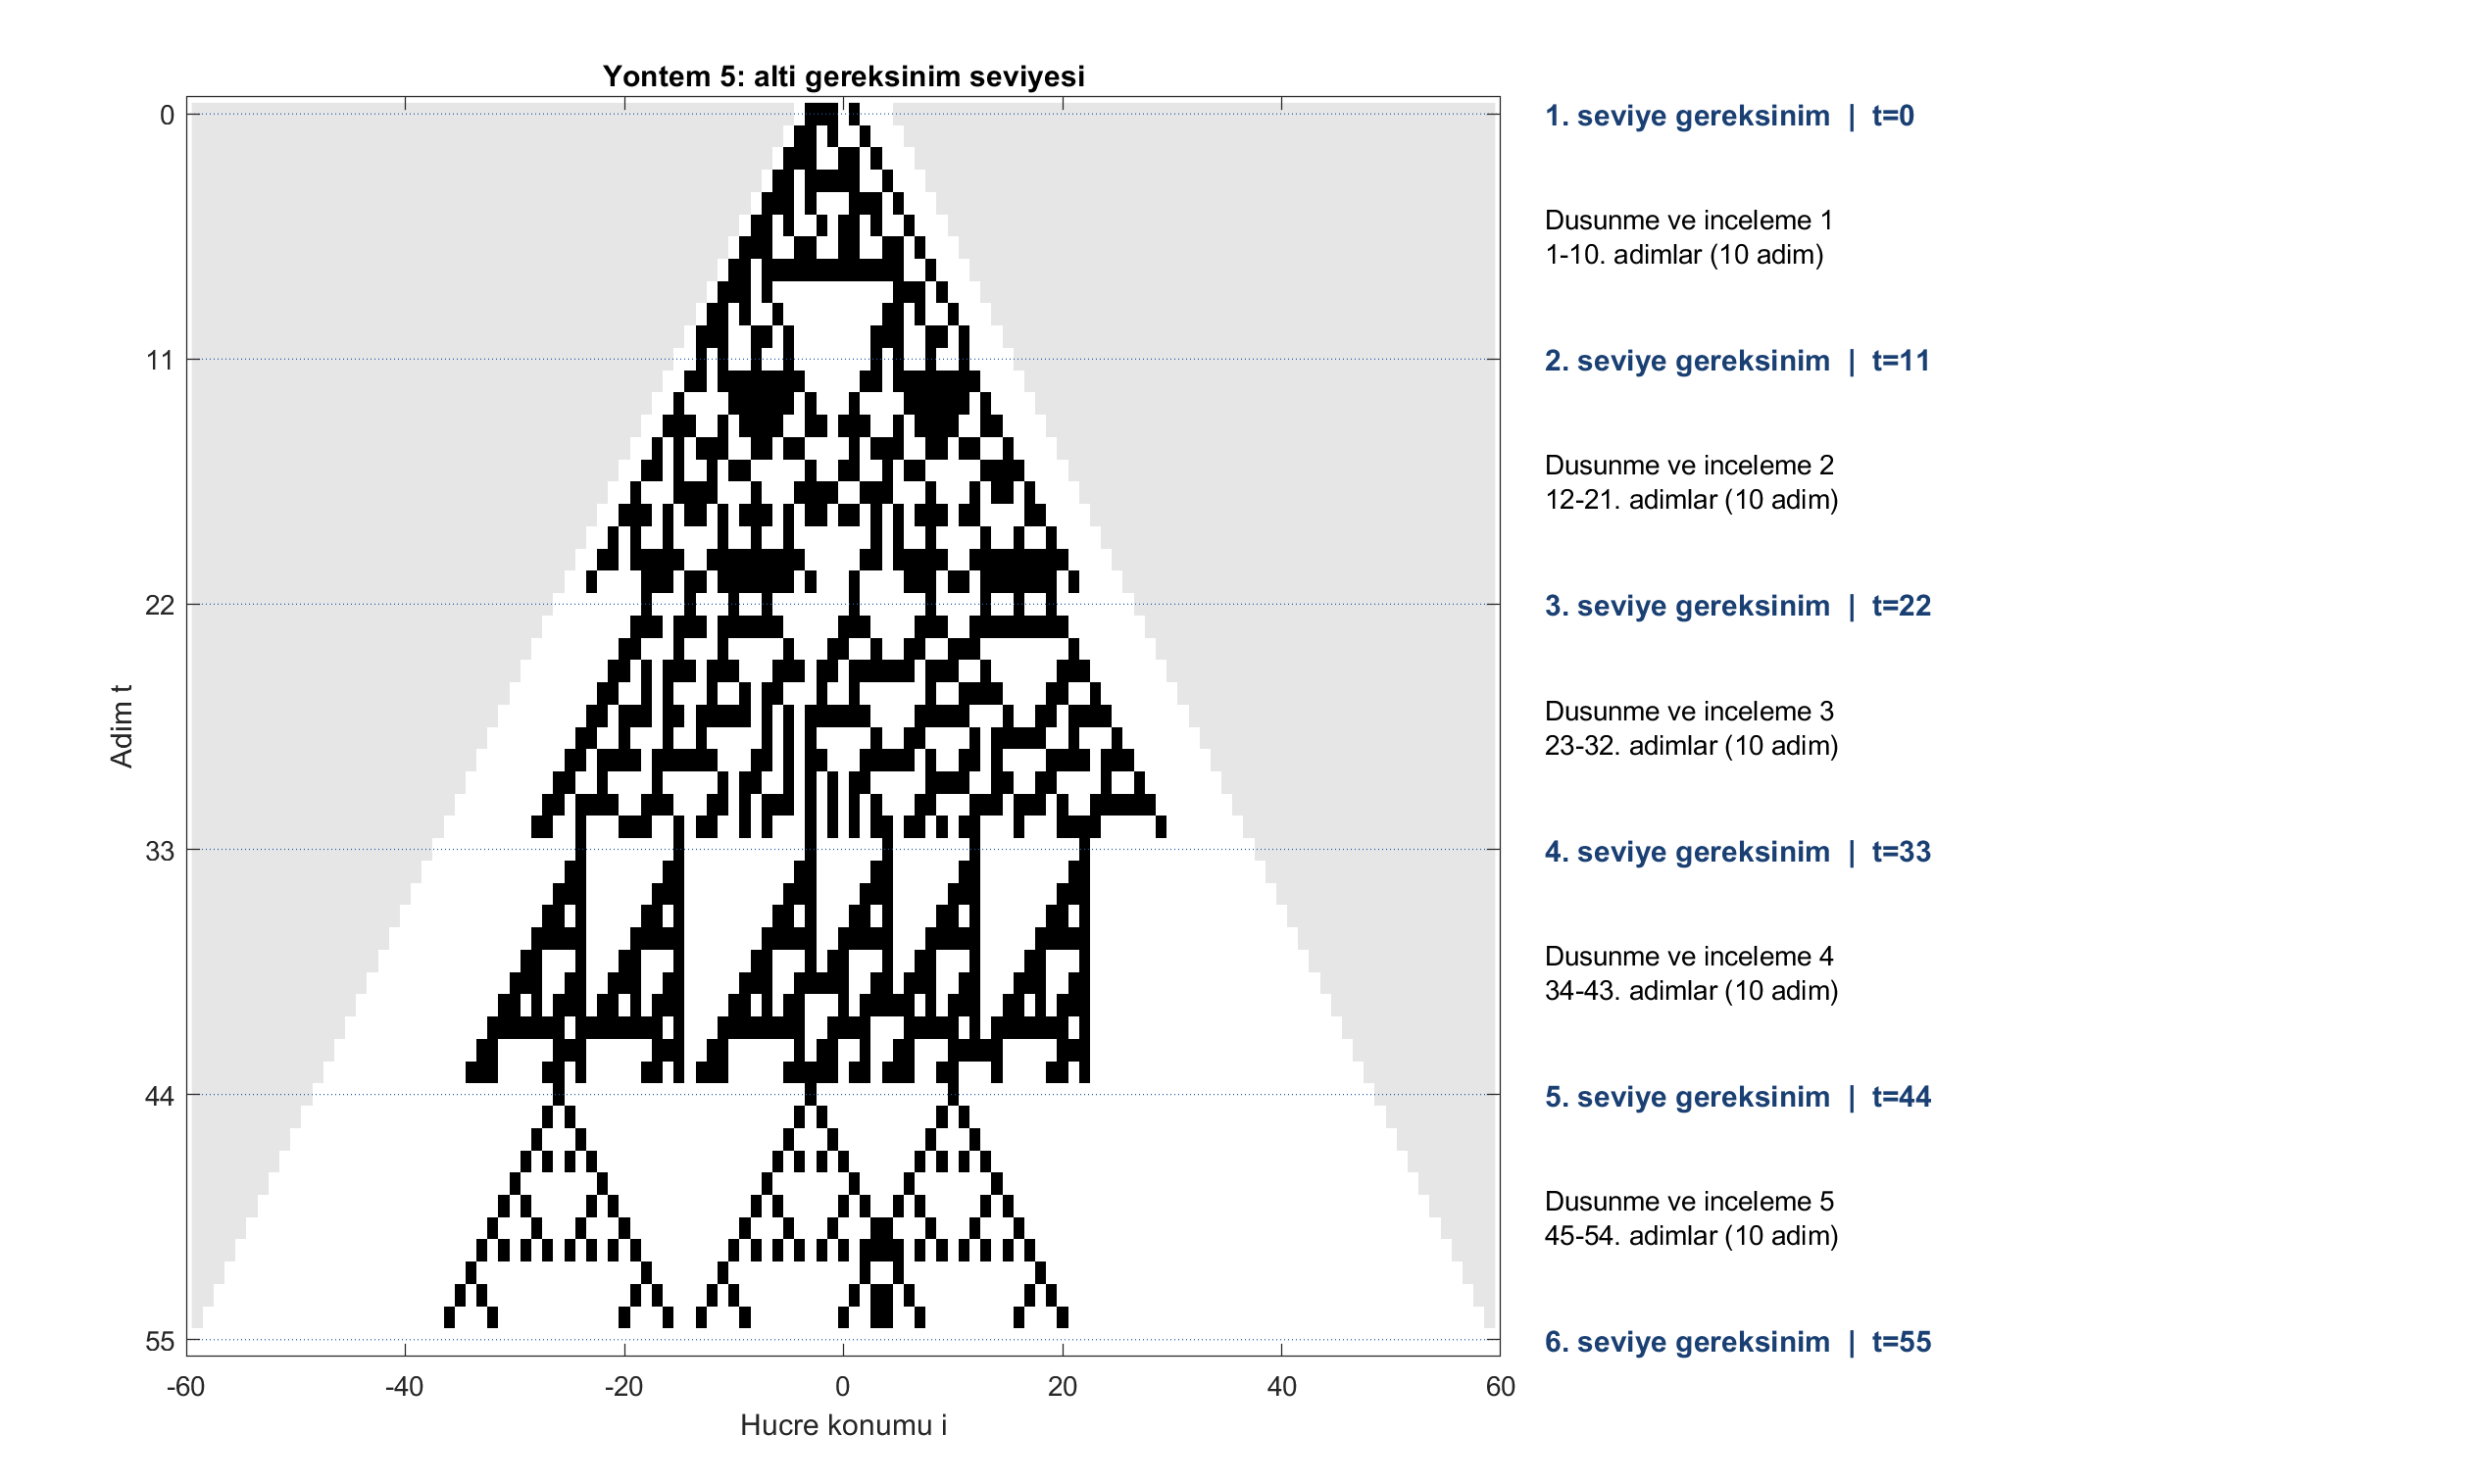
\includegraphics[width=\linewidth]{assets/image_5.png}\end{center}
\small Mavi kesikli çizgiler seviye satırlarını, sağdaki başlıklar on adımlık düşünme dönemlerini işaretler. Siyah 1, beyaz 0; gri alan ölçüm penceresi dışıdır. İşaretleme çizgileri hesaplanan hücrelere dahil değildir.\normalsize
\begin{center}\small\begin{tabular}{cr p{128mm}}\toprule Seviye & $t$ & Bu seviyede kayda geçen gereksinim kararı\\\midrule
2 & 11 & Kavram incelemesi: 16 paket içinden ilk 12 aday tutulur. \\
3 & 22 & Masaüstü prototip: ilk 8 aday tutulur. \\
4 & 33 & Mekanizma prototipi: ilk 4 aday tutulur. \\
5 & 44 & İşlev kıyası: son iki aday 1011 ve 1010 kalır. \\
6 & 55 & Tam çevrim testi ve seçim: 1011 kalır; dört kabul kaydı geçer. \\
\bottomrule\end{tabular}\end{center}

\page{Yöntem 5/5 | Sayısal analiz}{Prototiplerle aday eleme: entropi değişimi}
\begin{center}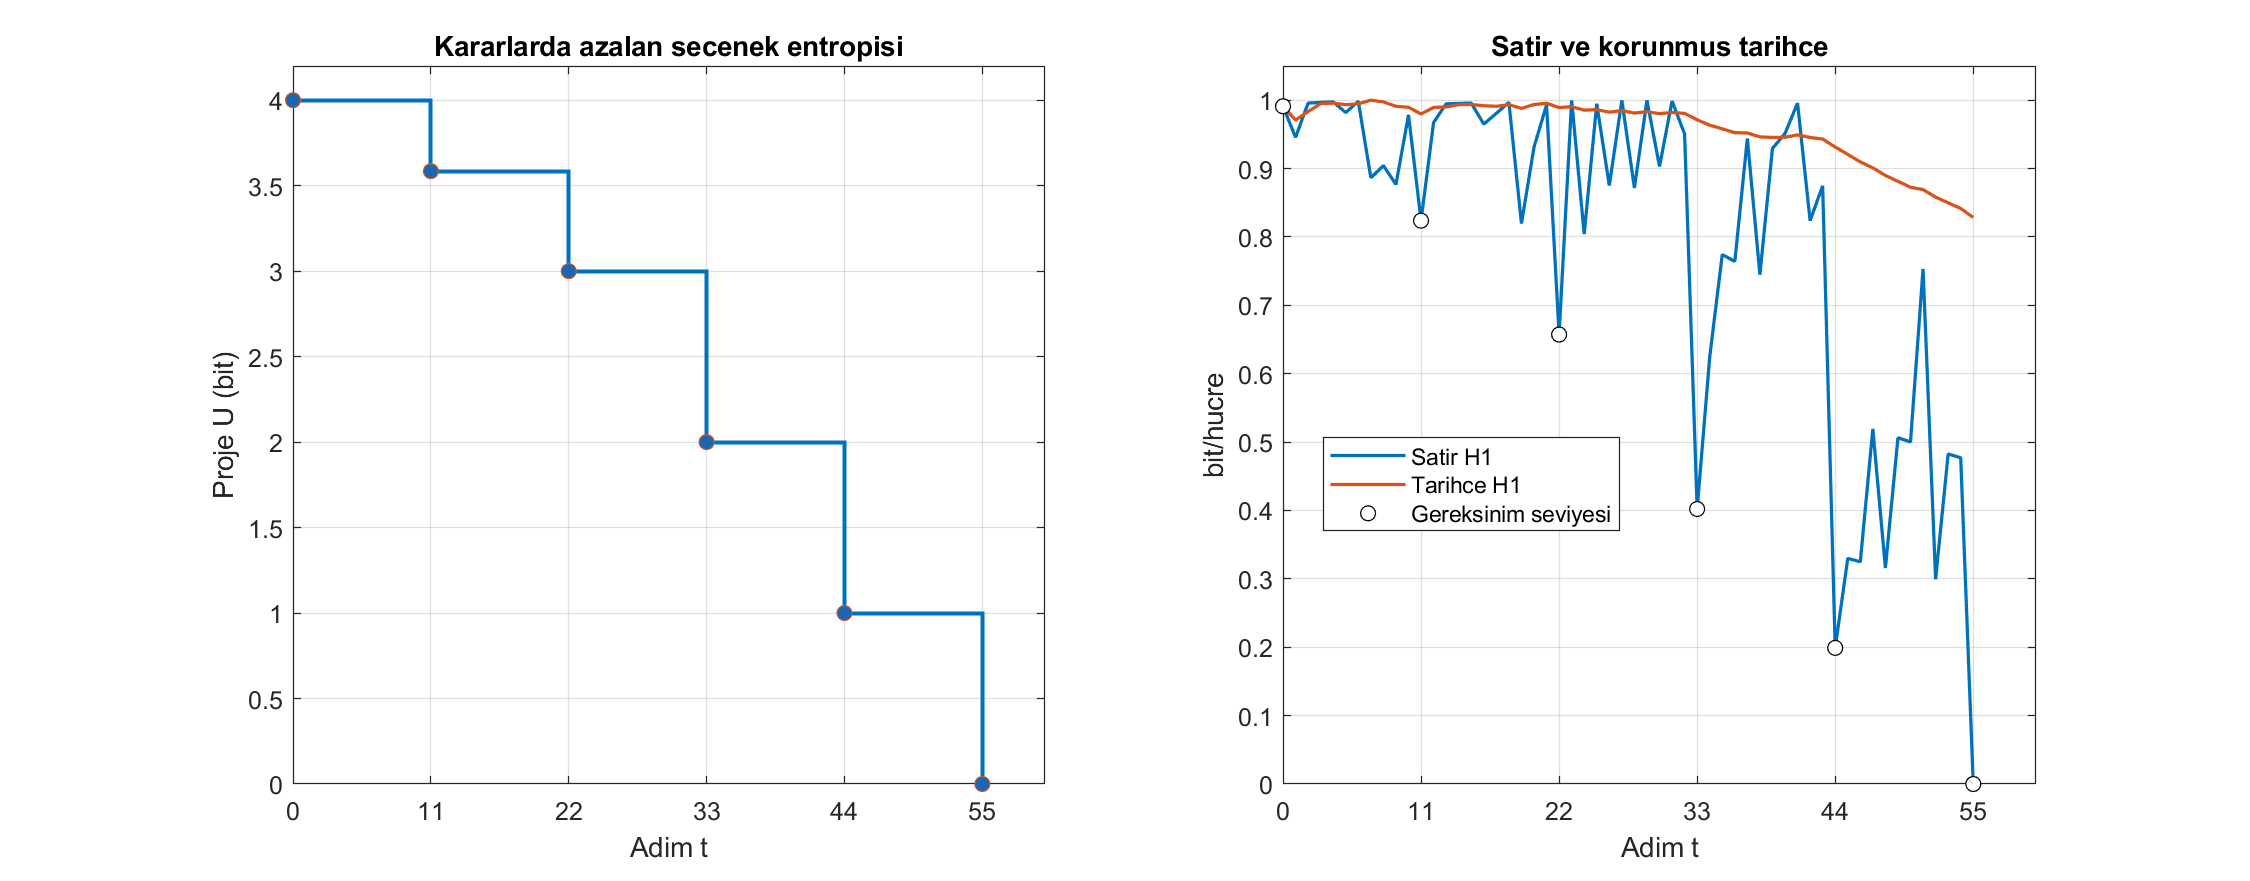
\includegraphics[width=\linewidth]{assets/entropy_5.png}\end{center}
\begin{center}\small\begin{tabular}{crrrrrr}\toprule Seviye & $t$ & Aday & Açık konu & Proje $U$ & Satır $H_1$ & Geçmiş $H_1$\\\midrule
1 & 0 & 16 & 4 & 4,0000 & 0,9911 & 0,9911 \\
2 & 11 & 12 & 4 & 3,5850 & 0,8238 & 0,9799 \\
3 & 22 & 8 & 4 & 3,0000 & 0,6573 & 0,9892 \\
4 & 33 & 4 & 3 & 2,0000 & 0,4022 & 0,9713 \\
5 & 44 & 2 & 1 & 1,0000 & 0,1990 & 0,9315 \\
6 & 55 & 1 & 0 & 0,0000 & 0,0000 & 0,8285 \\
\bottomrule\end{tabular}\end{center}
\textbf{Karar anının kontrolü.} Aynı genişlikteki geçici satır ile karar sonrası satır aşağıda karşılaştırılır. $\Delta H=H_{\rm ön}-H_{\rm son}$ pozitif olmalıdır.
\begin{center}\small\begin{tabular}{rrrrrr}\toprule $t$ & $H_{\rm ön}$ & Hedef $H^*$ & $H_{\rm son}$ & $\Delta H$ & Azalan işaret\\\midrule
11 & 0,9629 & 0,8630 & 0,8238 & 0,1391 & 4 \\
22 & 0,9977 & 0,6894 & 0,6573 & 0,3404 & 19 \\
33 & 0,9427 & 0,4382 & 0,4022 & 0,5405 & 21 \\
44 & 0,8670 & 0,2011 & 0,1990 & 0,6680 & 25 \\
55 & 0,4717 & 0,0000 & 0,0000 & 0,4717 & 12 \\
\bottomrule\end{tabular}\end{center}
\textbf{Yorum.} Aday sayıları 16, 12, 8, 4, 2, 1 olarak daralır. Bu yöntem tek bir konuya değil, bütün paketlerin karşılaştırılmasına dayanır. İlk elemeler sırasında dört konunun tamamı açık kalabilir; konu sayısı ile aday entropisi bu nedenle farklıdır.

Her elde kalan kümede eş ağırlık varsayılır: $U=\log_2 M$. Örneğin ikinci seviyede $U=\log_2 12=3{,}5850$ bittir.
\page{Beş yöntemin karşılaştırılması}{4\quad Altıncı seviyeye hangi yoldan ulaşılıyor?}
\begin{center}\small\begin{tabular}{lrrrrrr}\toprule
Yöntem & S1 & S2 & S3 & S4 & S5 & S6\\\midrule
Sıralı karar & 4,0000 & 3,7219 & 3,0000 & 2,0000 & 1,0000 & 0,0000 \\
Paralel çalışma & 4,0000 & 3,4439 & 2,0000 & 1,7219 & 1,0000 & 0,0000 \\
Kısıt yayılımı & 4,0000 & 3,7219 & 2,7219 & 1,7219 & 1,0000 & 0,0000 \\
Kanıt güncelleme & 4,0000 & 2,8877 & 1,2910 & 0,4587 & 0,1470 & 0,0000 \\
Prototip eleme & 4,0000 & 3,5850 & 3,0000 & 2,0000 & 1,0000 & 0,0000 \\
\bottomrule\end{tabular}\end{center}
Tablo proje karar entropisini bit cinsinden gösterir. Bütün yöntemler aynı
16 paketle ve $U=4$ ile başlar; altı seviyenin tamamında sıkı azalışla
$U=0$'a ulaşır. Her yöntem için beş karar satırındaki renk entropisi de
önceki gereksinim seviyesinden ve hemen önceki düşünme satırından düşüktür.

\textbf{Düşünme sırasında renk entropisi dalgalanabilir.} On adımlık
dönemlerde desen yayılır, bazı yerlerde birleşir veya iptal olur. Bu yüzden
$H_1$'in her düşünme adımında artması istenmemiş ve zorlanmamıştır.
Azalış koşulu özellikle gereksinim seviyelerine geçişte uygulanmıştır.

\textbf{Konu sayısı ile olasılık belirsizliği ayrılır.} Kanıt yönteminde
ikinci--beşinci seviyelerde açık konu sayısı dört kalır, fakat olasılık
dağılımı hedef pakete yoğunlaşır. Prototip yönteminde adaylar elenirken
konular farklı birleşimlerde açık kalabilir. Bu yüzden yalnız siyah sayısı
veya açık konu sayısıyla proje belirsizliği ölçülmez.

\textbf{Azalış iki farklı kaynaktan gelir.} $U$'daki azalış karar, kanıt
veya eleme girdisinden gelir. $H_1$'deki garantili azalış ise bu girdiye
bağlanan açık yeniden kodlama kuralından gelir. Bu iki sayının birlikte
azalması, birinin diğerini deneysel olarak doğruladığı anlamına gelmez.

\textbf{Ortak kapanış.} Altıncı seviyede tek paket 1011 kalır; $U=0$,
açık konu sayısı 0, başarılı kabul kaydı 4/4 ve son satır $H_1=H_2=0$ olur.
Geçmiş satırlar değiştirilmez. Proje kapanışı bu kapsam içindir; yeni bir
gereksinim veya başarısız test, ilgili kararların yeniden açılmasını gerektirir.

\textbf{Araştırmada kullanım.} Bu deney, istenen altı seviyeli görsel akışın
hesaplanabilir bir örneğidir. Gerçek tasarım çalışmasında her kapı için
hangi inceleme çıktısının hangi olasılığı veya adayı değiştirdiği kaydedilmelidir.
Yöntemlerin hız, maliyet veya başarı üstünlüğü bu simülasyondan çıkarılamaz.

\page{Yeniden üretim ve doğrulama}{5\quad MATLAB ve TeX kaynakları}
Kaynak paketini açtıktan sonra MATLAB komutu:
\begin{verbatim}
build_six_levels(fullfile(pwd,'assets'))
\end{verbatim}
MATLAB R2018b ile çalıştırılmıştır; ek toolbox gerekmez. Her yöntem için
işaretli resim ve entropi grafiği PNG/FIG biçiminde, tam 56 satır CSV olarak
üretilir. Adayların 16 sütunlu olasılık tablosu ayrıca saklanır.

\begin{center}\small\begin{tabular}{p{66mm}p{84mm}}\toprule
Dosya & İçerik\\\midrule
\texttt{build\_six\_levels.m} & On adımlık dönemler, beş karar kapısı, yeniden kodlama\\
\texttt{pattern\_entropy.m} & Tekli/ikili hücre desenlerinin entropisi\\
\texttt{assets/method\_N.csv} & 56 adımın bit dizisi, seviye, entropi ve karar verileri\\
\texttt{assets/posterior\_N.csv} & Her adımda 16 paket için olasılıklar\\
\texttt{assets/image\_N.png} & Seviyeler ve düşünme dönemleri işaretli resim\\
\texttt{assets/entropy\_N.png} & Adıma göre entropi eğrileri\\
\texttt{alti\_seviye\_gereksinim.tex} & Bu raporun düzenlenebilir kaynağı\\\bottomrule
\end{tabular}\end{center}

\textbf{Bağımsız doğrulama.} Python ile 280 satır ve 4480 aday olasılığı
yeniden hesaplanmıştır. Bütün bit dizileri; hücre sayıları; $H_1$, $H_2$,
geçmiş entropisi, proje entropisi, hedef entropi ve karar öncesi entropi
$10^{-12}$ mutlak tolerans içinde MATLAB ile eşleşmiştir. 25 karar kapısında
sıkı azalış ve beş son durumda sıfır koşulları kontrol edilmiştir.

CSV dosyalarında karar olmayan satırların karar öncesi/hedef entropisi
\texttt{NaN}'dır: o adımda karar işlemi yoktur. Kural alanındaki -1,
başlangıç veya karar satırını belirtir; bir hücresel otomat numarası değildir.

TeX derlemesi için aynı komutu iki kez çalıştırın:
\begin{verbatim}
xelatex -interaction=nonstopmode -halt-on-error
    alti_seviye_gereksinim.tex
\end{verbatim}
Komut tek satırda yazılır. XeLaTeX ve Cambria, Calibri, Consolas yazı tipleri
kullanılır. MATLAB parametreleri değişirse yalnız şekiller değil, rapordaki
sayısal tablolar ve yorumlar da yeni sonuçlara göre güncellenmelidir.

\textbf{Kavramsal dayanak.} S. Wolfram'ın (2023) \emph{Computational
Foundations for the Second Law of Thermodynamics} yazısındaki yerel hesaplama
ve gözlemci tartışması görsel modele ilham verir. Buradaki altı seviye,
karar olasılıkları ve entropi kontrollü özetleme bu rapora özgü model tercihleridir.
\end{document}
